\section{Metodología para localizar de forma resiliente la fuente de un campo escalar con enjambres robóticos}

%%%%%%%%%%%%%%%%
% Introducción %
%%%%%%%%%%%%%%%%

La búsqueda de fuentes en campos escalares (\textit{Source-Seeking}) se considera un problema fundamental dentro del campo de la robótica de enjambres, debido a su enorme potencial para resolver algunos de los desafíos más actuales \cite{brambilla2013swarm}. El objetivo consiste en que un equipo de robots sea capaz de coordinarse efectivamente para detectar y rodear fuentes de, por ejemplo, productos químicos, contaminación o señales de radio. Resolver este problema permitiría llevar a cabo misiones de persistencia (24/7) en áreas extensas, cambiando drásticamente la forma que tenemos actualmente de monitorizar el medio ambiente, realizar operaciones de búsqueda y rescate, o ejecutar agricultura de precisión \cite{ogren2004cooperative, kumar2004robot, mcguire2019minimal, li2006moth,twigg2012rss}. 

Como ya comentamos en la introducción, gracias a su alta resiliencia, los enjambres de robots se encuentran hoy en día entre los sistemas multiagente más prometedores. Su naturaleza les permite preservar la funcionalidad frente a condiciones adversas inesperadas y perturbaciones desconocidas. En el contexto de búsqueda de fuentes, con un enjambre se podría asegurar, por ejemplo, que el equipo de robots encuentre la fuente aunque ciertos agentes desaparezcan durante la misión. No obstante, aunque inicialmente todo esto suena muy bien, garantizar formalmente el rendimiento de este tipo de soluciones, mientras se mantiene su viabilidad práctica, no es tarea sencilla. En el mundo real, todo algoritmo aplicable a la robótica de enjambres debe de tener en cuenta dinámicas de robots realistas, dispositivos de comunicación y la escalabilidad \cite{dorigo2021swarm}.

\vspace{0.4cm}

\begin{figure}[h!]
    \centering
    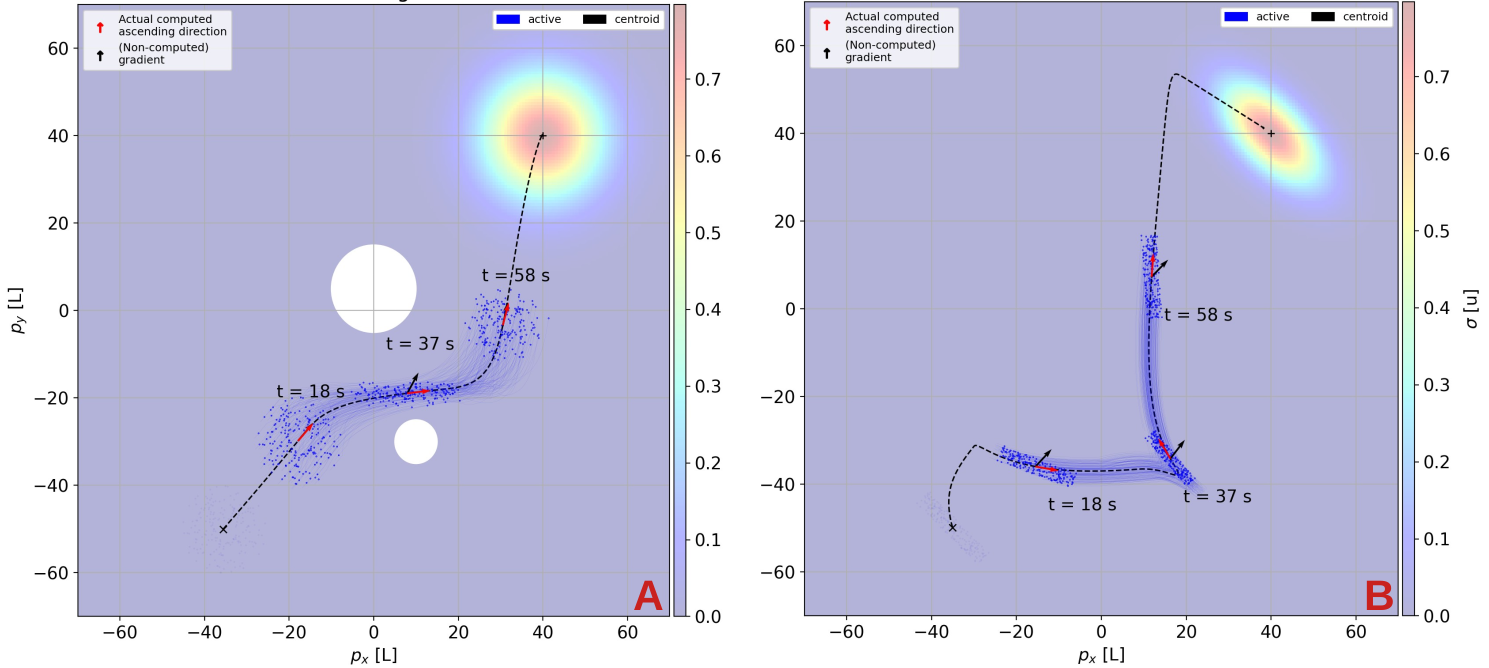
\includegraphics[trim={0 0cm 0 0cm}, clip, width=1\textwidth]{fig/ss_intro.png}
    \caption{En esta figura tenemos a dos enjambres de 200 robots con dinámica de integrador simple utilizando nuestro algoritmo de \textit{source-seeking} para ajustar su dirección de movimiento mediante modificaciones en la geometría de su formación. En (\textbf{A}), el enjambre \textbf{evita los obstáculos} al pasar de una formación circular a otra rectangular. En (\textbf{B}), el enjambre \textbf{rota} 90º su \textbf{dirección de movimiento} realizando una rotación equivalente de su formación rectangular.}
    \label{fig: SS_intro}
\end{figure}

\newpage

En este trabajo, proponemos un algoritmo resiliente y escalable capaz de coordinar a un equipo de robots para alcanzar la fuente de un campo escalar. Demostraremos, de forma rigurosa, cómo el enjambre determina con medidas locales de intensidad una \textbf{dirección de ascenso}, en lugar del gradiente, con la que guiar al centroide del enjambre hacia la fuente. Seguir esta estrategia, nos permite dotar al algoritmo de una gran \textbf{flexibilidad}, pues no se requiere de una formación específica para el enjambre de robots. Veremos que, gracias a esta caracterísca, la dirección de ascenso calculada reacciona a la relación entre la geometría de la formación y el campo escalar; por lo tanto, actuando únicamente sobre la distribución del enjambre o la forma del campo, seremos capaces de maniobrar al equipo de robots mientras continúan aproximándose simultáneamente a la fuente. Dicho de otro modo, podremos modular indirectamente la dirección de movimiento del enjambre durante la misión para, por ejemplo, evitar obstáculos o adaptarnos a otros factores ambientales (ver \autoref{fig: SS_intro}).

Dicha flexibilidad, será también la encargada de aportar \textbf{resiliencia y robustez} al algoritmo. En caso de que ciertos robots desaparezcan o se unan al enjambre, el algoritmo seguirá funcionando, ya que podrá manejar perfectamente la formación resultante. Por esta misma razón, tampoco será un problema gestionar la fusión y división de enjambres de robots, lo que permitirá, por ejemplo, fusionar dos equipos de robots en rumbo de colisión y dividirlos una vez sus direcciones de ascenso individuales ya no estén en conflicto.

% Una vez que se calcula la dirección de ascenso para el centroide, la estrategia a seguir para alinear al enjambre con ella variará en función de la dinámica de los robots que lo componen. En este trabajo analizaremos lo que sucede con el integrador simple y el uniciclo, donde podremos utilizar el mismo controlador presentado en la metodología anterior para alinear a los robots con el campo vectorial de guiado.

%%%%%%%%%%%%%%%%%%%%%%%%
% Fundamentos teóricos %
%%%%%%%%%%%%%%%%%%%%%%%%

\subsection{Fundamentos teóricos}

\subsubsection{Algoritmos existentes de source-seeking: Virtudes y defectos}

Los algoritmos del estado del arte que abordan el problema de \textit{source-seeking} ofrecen una serie de virtudes y defectos. No existe la solución perfecta, y por supuesto nuestro algoritmo no es una excepción. Por esta razón, antes de comentar a analizarlo detalladamente, procederemos a contextualizarlo revisando algunas las soluciones existentes. Es decir, resumiremos las posibilidades que otros algoritmos de la literatura tienen para ofrecer, de modo que el lector pueda evaluar sus virtudes y defectos en comparación con nuestra solución. Particularmente, nos centraremos en hablar sobre la adaptabilidad de la formación de robots, la consideración de dinámicas que se ajusten a robots realistas, el rendimiento anticipado en términos de distancia recorrida o trayectorias previstas suaves, o los requisitos de comunicación, como la topología y el ancho de banda.

El primer método ampliamente utilizado se centra en la \textbf{estimación del gradiente y el Hessiano}, donde podemos encontrar algunas variaciones. Por ejemplo, los autores en \cite{rosero2014cooperative, barogh2017cooperative} estiman el gradiente de los robots en sus posiciones de forma distribuida, y el acuerdo sobre la dirección común a seguir se obtiene aplicando un controlador de formación basado en la distancia que mantiene la cohesión del enjambre. Sus resultados se demuestran con robots modulados como puntos cinemáticos (integradores simples o dobles), y dejan ver que la estimación del gradiente se vuelve poco confiable si al menos un grupo de robots vecinos muestra una forma degenerada, como una línea, en el plano 2D. 

Los autores en \cite{brinon2015distributed, brinon2019multirobot} estiman el gradiente y el Hessiano de un enjambre de robots en el centroide de una \emph{formación circular}. Su técnica permite el uso de robots con dinámica de uniciclo; no obstante, el algoritmo es muy rígido, ya que necesariamente la geometría de la formación ha de ser circular, o una esfera en 3D. La misma formación circular resulta de aplicar el algoritmo propuesto en \cite{fabbiano2016distributed}, donde los robots también se modelan como uniciclos; sin embargo, en este caso los agentes no necesitan medir sus posiciones relativas, sino sus orientaciones relativas. Finalmente, relacionado con la técnica del gradiente, pero asumiendo que se conoce el campo, en \cite{ogren2004cooperative} podemos encontrar uno de los algoritmos más pioneros.

La \textbf{búsqueda de extremos} es otra técnica ampliamente utilizada para el problema de \textit{source-seeking}, como se analiza en \cite{li2020cooperative,cochran2009nonholonomic}. En estos trabajos, se fuerza a los robots (normalmente solo uno) a realizar movimientos periódicos para realizar una estimación del gradiente no basada en modelos. El método tiene éxito con dinámicas no holonómicas; no obstante, en caso de varios robots, es posible que necesiten intercambiar parámetros estimados y, según la acción de control resultante, las trayectorias finales de los robots podrían alejarse de las deseadas, ya que suelen ser largas y tortuosas con giros bruscos.

Todos los algoritmos mencionados anteriormente para la búsqueda de fuente requieren comunicación (principalmente distribuida), es decir, los robots comparten la intensidad del campo escalar. No obstante, los autores en \cite{al2021distributed} ofrecen una solución elegante que no requiere compartir la intensidad del campo entre los robots. Sin embargo, es necesario conocer la posición del centroide del enjambre de robots, y un algoritmo para su estimación distribuida podría requerir comunicación dentro del equipo. El método que proponen utiliza un algoritmo de \textbf{análisis de componentes principales basado en consenso}, y los robots modulan sus movimientos centrados únicamente en sus mediciones instantáneas del campo; por lo tanto, la formación (variable en el tiempo) de los robots durante la misión está determinada por sus posiciones iniciales y el campo escalar. En otras palabras, la formación no está bajo control.

Concluimos esta breve revisión de la literatura haciendo referencia a un problema muy relacionado, el problema de \textbf{cobertura con sensores móviles} \cite{cortes2004coverage}. Los algoritmos que abordan este escenario son particularmente buenos para rodear más de una fuente simultáneamente con un enjambre de robots. Mayoritariamente, se basan en explotar la partición de un área con celdas de Voronoi. Sin embargo, hasta ahora dicho rendimiento conlleva un precio más alto que las soluciones típicas de \textit{source-seeking}. En estos algoritmos, el robot (o enjambre) necesita la información (densa o continua) del campo escalar dentro de su celda correspondiente y, además, su configuración eventual depende de la forma de dicha celda, que ha de ser fija o conocida de antemano.


\subsubsection{Notación general}

Consideremos un equipo de $N \in \mathds{N}$ robots, donde la posición del robot $i \in \{1,\dots,N\}$ en el espacio cartesiano se representa por $p_i \in \mathds{R}^m$, donde $m \in \{2,3\}$ es la dimensión de dicho espacio. Definimos $p\in\mathds{R}^{mN}$ como el vector apilado que contendrá las posiciones de todos los robots que conforman al enjambre. 

Cuando trabajemos con múltiples enjambres, definiremos $N_c \in \mathds{N}$ como el número de \textbf{equipos de robots}. En estos casos, denotaremos al número de robots en el $k$-ésimo equipo como $N_k$, y la posición del $i$-ésimo robot en el $k$-ésimo grupo como $p_i^k \in \mathds{R}^m$. Téngase en cuenta que omitiremos el superíndice $k$ por claridad si solo hay un equipo. En cada enjambre, habrá una \textbf{unidad de cálculo} que recopilará la información de todos agentes dentro del equipo.

\vspace{1cm}

\begin{figure}[!h]
\centering
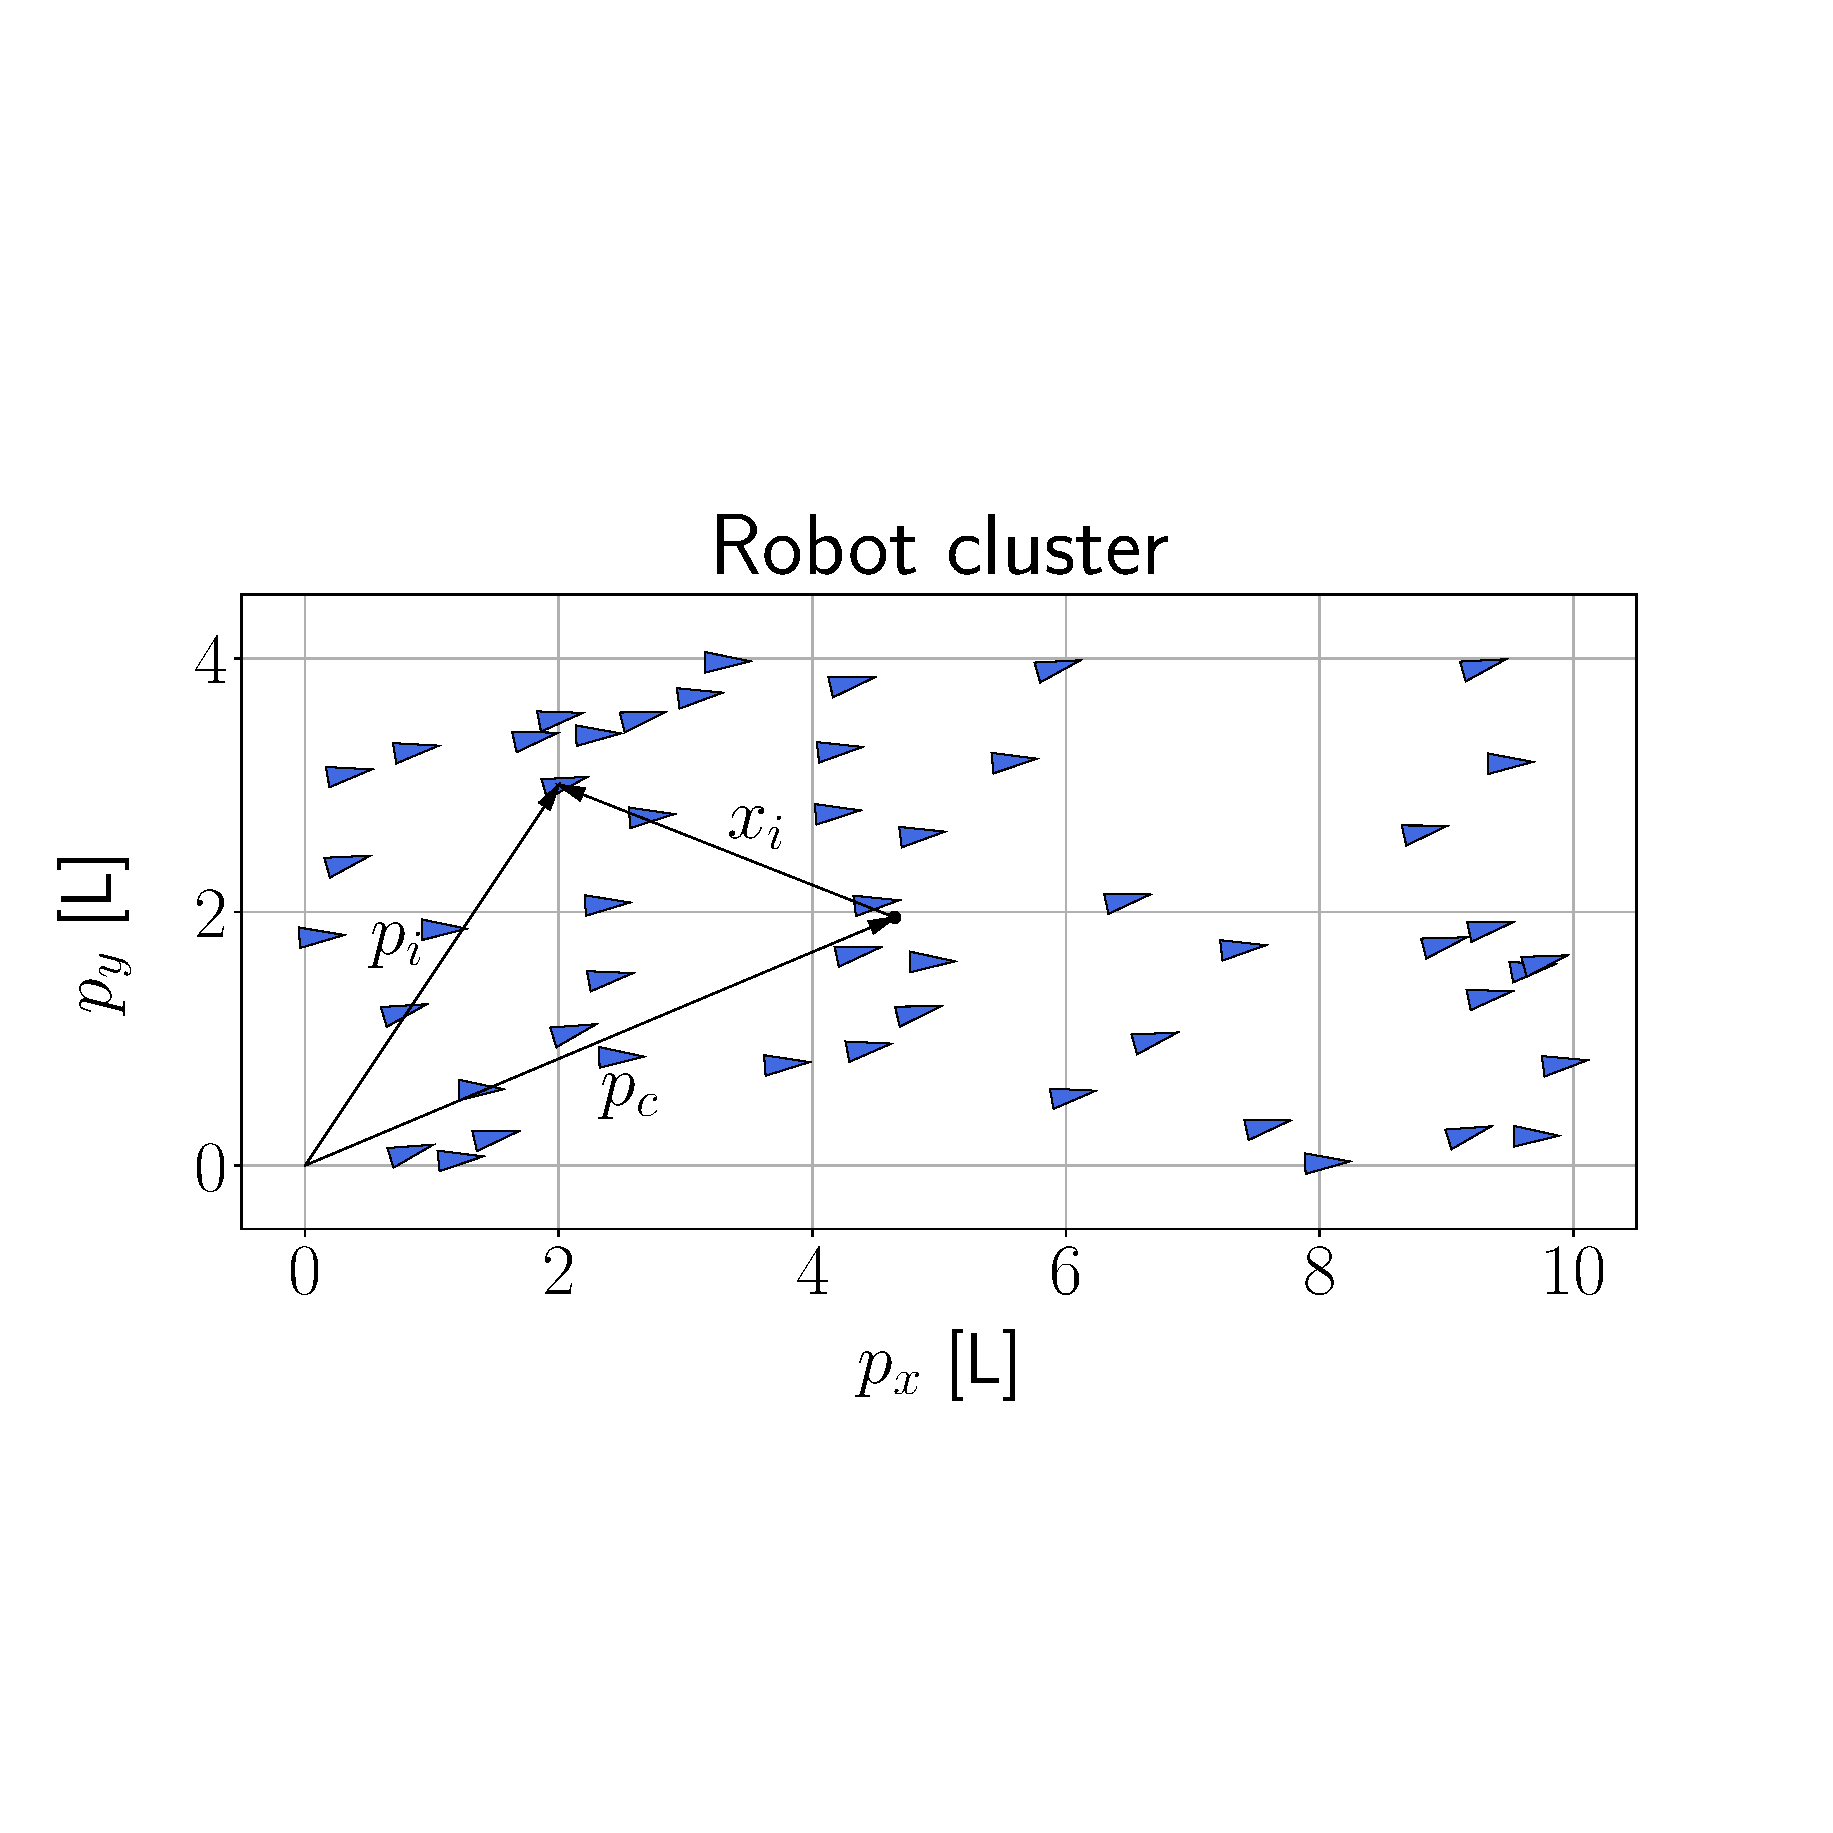
\includegraphics[trim={0 7cm 0 9.6cm}, clip, width=0.8\columnwidth]{./fig/SS_pcxi.eps}
\caption{Despliegue $x$ de un enjambre de robots con centroide en $p_c$. El vector $p_i$ representa la posición de cada agente con respecto al sistema de referencia y $x_i$ su posición con respecto al centroide.}
\label{fig: deployment}
\end{figure}

Nuestro algoritmo de \textit{source-seeking} lo contrastaremos con robots que simularán la dinámica de integrador simple y uniciclo. En el primer caso, los agentes pueden seguir directamente la velocidad guía en 2D y 3D. Nos obstante, para el caso de los uniciclos, será necesario utilizar un controlador secundario para alinear la dirección del robot con la dirección de ascenso. Se puede demostrar que dicho controlador puede ser muy similar al utilizado en la metodología anterior para alinear a los agentes con el GVF. Para más información, consultar \cite{tfg_antonio}. 

Definimos el centroide de un equipo como $p_c := \frac{1}{N}\sum_{i=1}^{N}p_i$. Por lo tanto, podemos escribir $p_i = p_c + x_i$, donde $x_i\in\mathds{R}^m$ para todo $i\in\{1,\dots,N\}$ describe cómo se distribuyen los robots alrededor de su centroide (ver Figura \ref{fig: deployment}).

\begin{definition} [Geometría del enjambre]
El vector apilado $x := \begin{bmatrix}x_1^T, \dots, x_N^T\end{bmatrix}^T \in \mathds{R}^{mN}$ denotará la geometría o formación del enjambre. Dicha geometría será \textbf{no degenerada} si los vectores $\{x_1^T, \dots, x_N^T\}$ generan el espacio $\mathds{R}^m$.
\end{definition}

Teniendo en cuenta esta definición, entonces es necesario imponer que $N > m \geq 2$ para que la geometría del enjambre no sea degenerada. La intensidad de una señal en todo el espacio puede describirse mediante un campo escalar de la siguiente manera.

\begin{definition} [Intensidad de un señal]
La intensidad de una señal es un campo escalar $\sigma: \mathbb{R}^m \to \mathbb{R}^+$, dos veces diferenciable y con todas sus derivadas hasta segundo orden acotadas globalmente. En nuestro caso, dicho $\sigma$ cuenta únicamente con \textbf{un máximo} en $p_\sigma$ y su gradiente en $a\in\mathbb{R}^m$ satisface que $\nabla\sigma(a) \neq 0 \iff a \neq p_\sigma$ y $\lim_{||a||\to\infty}\sigma(a) \to 0$.
\end{definition}

Algunas de las señales que se ajustan a esta definición son las distribuciones Gaussianas, o todas aquellas señales que disminuyen desde la fuente de acuerdo con la ley de potencia $x^{-\alpha}$, con $2 \leq \alpha \leq 3$, modelo que comienza a ser aplicable después de considerar una distancia mínima fija $x_{\text{min}}$ desde el origen \cite{clauset2009power}. La intensidad de este tipo de señales se puede representar, por ejemplo, como el módulo del campo electromagnético, la concentración de un contaminante o la radiación de calor. En particular, resulta interesante tener en cuenta las distribuciones cuadráticas (leyes de potencia $x^{-2}$), o el logaritmo de una distribución Gaussiana, pues son muy relevantes dentro del mundo físico que observamos.

En este trabajo, definiremos el gradiente como un vector columna $\nabla\sigma(\cdot) \in \mathds{R}^m$. Véase que, según nuestra definición de señal, tenemos que

\begin{equation} \label{eq_grad_hess_bound}
\|\nabla\sigma(a)\| \leq K \quad \text{y} \quad \|H_\sigma(a)\| \leq 2M, \quad \forall a\in\mathds{R}^m,
\end{equation}

donde $K, M\in\mathds{R}^+$, y $H_\sigma$ es el Hessiano del campo escalar $\sigma$, es decir, $H_\sigma(a)\in\mathds{R}^{m\times m}$; por lo tanto, a partir de la expansión de la serie de Taylor de $\sigma$ en $a\in\mathds{R}^m$ \cite[Teorema 5.15]{WalterRudin1976Principles}, se sigue que

\begin{equation} \label{eq: stay}
| \sigma(a) - \sigma(b) - \nabla\sigma(a)^T(a-b) | \leq M \|a -b\|^2, \quad \forall b\in\mathds{R}^m.
\end{equation}

\subsection{Teoría de Grafos}
Los algoritmos que proponemos para resolver el problema de \textit{source-seeking} y estimar el centroide de un equipo van a ser implementados de forma distribuida. Por lo tanto, necesitamos introducir algunas nociones de Teoría de Grafos \cite{bullo2020lectures} para poder definir las relaciones entre los robots de manera precisa. Consideremos un grupo de $N$ robots, entonces un \textbf{grafo} $\mathcal{G} = (\mathcal{V}, \mathcal{E})$ consta de dos conjuntos no vacíos: el conjunto de nodos $\mathcal{V} = \{1,\dots,N\}$ donde cada nodo $i$ corresponde al robot $i$, y el conjunto ordenado de aristas $\mathcal{E} \subseteq (\mathcal{V}\times\mathcal{V})$ que define las comunicaciones o percepciones entre pares de robots diferentes. Para una arista arbitraria $\mathcal{E}_k = (\mathcal{E}_k^{\text{tail}},\mathcal{E}_k^{\text{head}})$, llamamos a su primer y segundo elemento la \textbf{cola} y la \textbf{cabeza} respectivamente. El conjunto $\mathcal{N}_i$ que contiene a los vecinos del nodo $i$ se define como $\mathcal{N}_i:=\{j\in\mathcal{V}:(i,j)\in\mathcal{E}\}$.

EN este trabajo, únicamente abarcaremos el caso especial de grafos \textbf{no dirigidos}, donde todas las aristas $\mathcal{E}_k$ se consideran \textbf{bidireccionales}; es decir, si $(i,j)\in\mathcal{E}$ entonces necesariamente $(j,i)\in\mathcal{E}$. Para un grafo no dirigido, elegimos solo una de estas dos direcciones arbitrarias entre los nodos $i$ y $j$, lo que nos permitirá construir la \textbf{matriz de incidencia} $B\in\mathbb{R}^{|\mathcal{V}|\times |\mathcal{E}|}$ de $\mathcal{G}$ de la siguiente manera:
\begin{equation}
	b_{ik} := \begin{cases}+1 \quad \text{si} \quad i = {\mathcal{E}_k^{\text{tail}}} \\
		-1 \quad \text{si} \quad i = {\mathcal{E}_k^{\text{head}}} \\
		0 \quad \text{en otro caso.}
	\end{cases}
	\label{eq: B}
\end{equation}
%Luego observamos que podemos construir un vector apilado $z\in\mathbb{R}^{m|\mathcal{E}|}$ de posiciones relativas en un grupo asociado al grafo $\mathcal{G}$ con $z = \overline B^Tp$.

Para un grafo no dirigido, la \textbf{matriz Laplaciana} $L\in\mathbb{R}^{|\mathcal{V}|\times |\mathcal{V}|}$ \cite[Capítulo 6]{bullo2020lectures} se puede calcular como
\begin{equation}
L = BB^T.
\label{eq: L}
\end{equation}
Si el grafo $\mathcal{G}$ es \textbf{conectado} \cite[Capítulo 3]{bullo2020lectures}, entonces la matriz Laplaciana $L$ tiene un único valor propio igual a cero, cuyo vector propio asociado es $\mathbf{1}_N$, ya que $B^T\mathbf{1}_N = 0$; por lo tanto, $L$ es semidefinida positiva.

\subsection{Formalización del problema}

Una vez introducida toda la notación necesaria, ya nos encontramos en disposición de formalizar el problema de \textit{source-seeking} con enjambres de robots.

\begin{problema}[\textit{Source-seeking} con enjambres de robots] \label{problema: ss}
Dada una señal $\sigma$, $N_c$ equipos de robots y una constante $\epsilon > 0$, encontrar acciones de control para todos los robots de manera que $\|p_c^k(t) - p_\sigma\| < \epsilon, \; \forall t \geq T, \; \forall k\in \{1,\dots,N_c\}$ para algún tiempo finito $T\in\mathds{R}^+$.
\end{problema}

%%%%%%%%%%%%%%
% Desarrollo %
%%%%%%%%%%%%%%

\subsection{Herramientas de \textit{source-seeking}}

En esta sección, presentaremos una serie de herramientas que nos permitirán diseñar una solución autónoma al problema de \textit{source-seeking}. Las herramientas que introduciremos en esta sección nos permitirán: calcular de forma distribuida la dirección de ascenso, analizar la observabilidad y sensibilidad de la dirección de ascenso con respecto a una formación $x$, coordinar a múltiples equipos para seguir una misma dirección de ascenso y, por último, realizar una estimación distribuida del centroide de un equipo utilizando a los robots que lo componen.


A continuación, resumiremos la información necesaria para que los robots implementen nuestra solución autónoma:

\begin{itemize}
    \item El robot $i$ mide la intensidad de la señal $\sigma(p_i)$.\\
    
    \item Dado un grupo codificado como un grafo $\mathcal{G}$, el robot $i$ mide en su sistema de coordenadas local la posición relativa $(p_i - p_j) = (x_i - x_j), \, (i,j)\in\mathcal{E}$. Ya veremos que, siempre y cuando $\mathcal{G}$ esté conectado, esta información es suficiente para estimar el centroide de forma distribuida.\\
    
    \item La unidad de cálculo del $k$-ésimo equipo necesita todas las $\sigma(p^k_i)$ y todas las posiciones relativas de los robots con respecto al centroide, es decir, $x_i^k = (p^k_i - p^k_c), \forall k\in{1,...,N_k}$. Por lo tanto, hay una topología en estrella para el cálculo de la dirección de ascenso. Si el número de robots de un grupo es muy grande, entonces éste se podrá dividir en una red arbitraria pero conectada de subgrupos con topología en estrella, para así calcular una dirección de ascenso de manera distribuida con un algoritmo de consenso estándar.\\
\end{itemize}

Cabe destacar que al enjambre nunca se le va a requerir conocer su posición con respecto a un sistema de referencia absoluto. Este es un factor muy importante, pues en la práctica hace que no sea necesario hacer uso de sistemas de geolocalización.

Dado el requisito de medir posiciones relativas entre robots, la formación geométrica deseada $x$ se puede lograr con controladores de formación basados en desplazamiento \cite{oh2015survey,sun2018circular,C1}. No entraremos mucho en detalle sobre cómo funcionan este tipo de controladores, pues no resultan ser una contribución original de este trabajo. No obstante, hay que tener en cuenta que será necesario su implementación para poder llevar ciertas herramientas de nuestro algoritmo autónomo de \textit{source-seeking} al mundo real.

A continuación, definiremos formalmente lo que entendemos por dirección de ascenso en un punto relativo a una señal $\sigma$.
\begin{definition}[Dirección de ascenso] \label{def: asc_dir}
Un vector no nulo $v \in \mathbb{R}^m$ es una dirección dirección de ascenso en un punto $p \in \mathbb{R}^m$ con respecto a una señal $\sigma:\mathbb{R}^m \to \mathbb{R}^{+}$ si y solo si $\nabla \sigma(p)^T v > 0$.
\end{definition}

%\item Las unidades de cómputo de los clústeres que siguen direcciones independientes y están en riesgo de colisión deben calcular una dirección de ascenso común para evitar colisiones. Esto se puede hacer con un algoritmo de consenso estándar en el que las unidades de cómputo solo comparten sus direcciones de ascenso.
%\item Para evitar colisiones entre clústeres cercanos, sus unidades de cómputo deben comunicarse para calcular una dirección de ascenso común. Necesitan compartir la siguiente información: sus direcciones de ascenso, su $\operatorname{max}_{1\leq i\leq N_k}{|x_i^k|}$, sus centroides y la velocidad del centroide en caso de que sean diferentes entre clústeres.

\newpage

% La dirección de ascenso
%%%%%%%%%%%%%%%%%%%%%%%%%%

\subsubsection{La dirección de ascenso}

Los autores en \cite{brinon2015distributed} demuestran que
\begin{equation}
\hat\nabla\sigma(p_c) = \frac{m}{ND^2}\sum_{i=1}^N \sigma(p_i)(p_i - p_c),
\label{eq: lara}
\end{equation}
es una estimación del gradiente de la señal, en el espacio 2D, en el centro de una circunferencia con radio $D$, si al menos tres robots están igualmente espaciados angularmente en la circunferencia. La misma expresión, también se emplea en \cite{brinon2019multirobot} para una distribución similar en una esfera 3D. A lo largo de esta subsección, veremos esta distribución simétrica particular es solo una condición suficiente para estimar el gradiente.

En los trabajos \cite{brinon2015distributed,brinon2019multirobot} se ha estudiado con detalle que \eqref{eq: lara} para distribuciones uniformes, en la circunferencia, no obstante, todavía no está claro si ésta sigue siendo una buena estimación del gradiente  para distribuciones genéricas. De hecho, sin aparentes cambios importantes, la expresión (\ref{eq: lara}) se puede extender significativamente admitiendo cualquier distribución genérica $x$. En particular, a lo largo de este trabajo demostraremos que bajo algunas condiciones, el vector

\begin{equation} \label{eq: Lsigma}
L_\sigma(p_c,x) = \frac{1}{ND^2}\sum_{i=1}^N \sigma(p_i)(p_i - p_c) = \frac{1}{ND^2}\sum_{i=1}^N \sigma(p_c + x_i)x_i,
\end{equation}

es una dirección de ascenso en $p_c$, donde ahora $D = \max_{1\leq i\leq N}{|x_i|}$. Esta expresión para la dirección de ascenso fue originalmente propuesta en \cite{tfg_antonio}, donde se presentaron una serie de resultados muy interesantes que han motivado en gran medida los análisis que llevaremos a cabo en este TFM.

Véase que $L_\sigma$ puede ser calculada por la unidad de cálculo de cada enjambre, ya que dispone de toda la información necesaria para ello. También conviene destacar que \eqref{eq: Lsigma}, a diferencia de \eqref{eq: lara}, es una función de una distribución genérica $x$, y que la dirección de ascenso no necesariamente aproxima el gradiente de la señal (es decir, posiblemente no es paralela al gradiente). Más adelante, veremos que esta propiedad es precisamente una ventaja que nos permitirá maniobrar al enjambre de robots manipulando únicamente $x$.

A continuación, aproximemos $\sigma(p_c + x_i)$ a una serie de Taylor de orden dos para $|x_{i}|$ \textbf{pequeños}, es decir, $\sigma(p_c + x_i) \approx \sigma(p_c) + \nabla\sigma(p_c)^Tx_i$, de modo que $L_\sigma(p_c,x) \approx L_\sigma^0(p_c,x) + L_\sigma^1(p_c,x)$, con


\begin{align} \label{eq: L1.1}
    L^0_\sigma(p_c,x) &= \frac{1}{ND^2}\sum_{i=1}^N \sigma(p_c) x_i, \nonumber \\
    L^1_\sigma(p_c,x) &= \frac{1}{ND^2}\sum_{i=1}^N \left(\nabla\sigma(p_c)^Tx_i\right)x_i, 
\end{align}



donde es fácil comprobar que $L^0_\sigma(p_c,x) = 0$ debido a la definición del centroide $p_c$.

\newpage

%---
\begin{rem}
La elección del factor $\frac{1}{ND^2}$ es irrelevante, ya que la propiedad importante de $L^1_\sigma$ es su dirección y no su magnitud. Sin embargo, $D^2$ hace que $L^1_\sigma$ tenga las mismas unidades que el gradiente, de modo que significan lo mismo físicamente [\emph{unidades de señal} / \emph{unidades de longitud}] = [U/L]. $N$ es simplemente un factor de promediación.
\end{rem}

El vector $L^1_\sigma$ es interesante porque \textbf{siempre} es una dirección de ascenso en el centroide $p_c$ (ver \autoref{fig: ss_lemma1}). Es decir, (\ref{eq: L1.1}) no requiere que se cumplan condiciones particulares, solo que la distribución $x$ no sea degenerada, tal y como se muestra en el siguiente resultado de \cite{tfg_antonio}:

\vspace{0.5cm}

\begin{lemma} [$L^1_\sigma(p_c,x)$ siempre es dirección de ascenso]
\label{le: l1}
Si la distribución $x$ es no degenerada y $p_c \neq p_\sigma$, entonces $L^1_\sigma(p_c,x)$ siempre es una dirección de ascenso en $p_c$ hacia el máximo $p_\sigma$ del campo escalar $\sigma$.
\end{lemma}
\begin{proof}
Si $L^1_\sigma$ es  siempre una dirección de ascenso, entonces debe cumplir $\nabla\sigma(p_c)^TL^1_\sigma(p_c, x) > 0$, y eso es fácil de comprobar ya que
\begin{equation}
\nabla\sigma(p_c)^TL^1_\sigma(p_c, x) = \frac{1}{ND^2}\sum_{i=1}^N |\nabla\sigma(p_c)^Tx_i|^2 \nonumber
\end{equation}
siempre es positivo si las posiciones relativas $x_i$ en la distribución $x$ abarcan $\mathbb{R}^m$ y $p_c \neq p_\sigma$.\\
\end{proof}

\vspace{0.2cm}

\begin{rem} \label{rem: L1}
Otra demostración comienza considerando $0 \neq b\in\mathbb{R}^m$ y el siguiente operador $\mathcal{L}(b, x) := \sum_{i=1}^N (b^Tx_i)x_i = \sum_{i=1}^N (x_ix_i^T)b$, y dado que $P(x) := \sum_{i=1}^N x_ix_i^T$ es definida positiva para $x$ no degenerada, entonces $b^T \mathcal{L}(b, x) = b^T P
Z b > 0$. Reemplazando $b$ por $\nabla \sigma(p_c)$, se puede demostrar el lema anterior. Además, si el resultado es $P = \lambda I_m$, donde $\lambda \in\mathbb{R}^+$, entonces $\mathcal{L}(b, x) = P b = \lambda b$, lo que significa que produce un vector paralelo a la entrada $b$. Veremos que si $x$ consta de los vértices de polígonos o poliedros, estas distribuciones tienen esta propiedad (es decir, Lema \ref{le: l1}).
\end{rem}

\begin{figure}[!h]
\centering
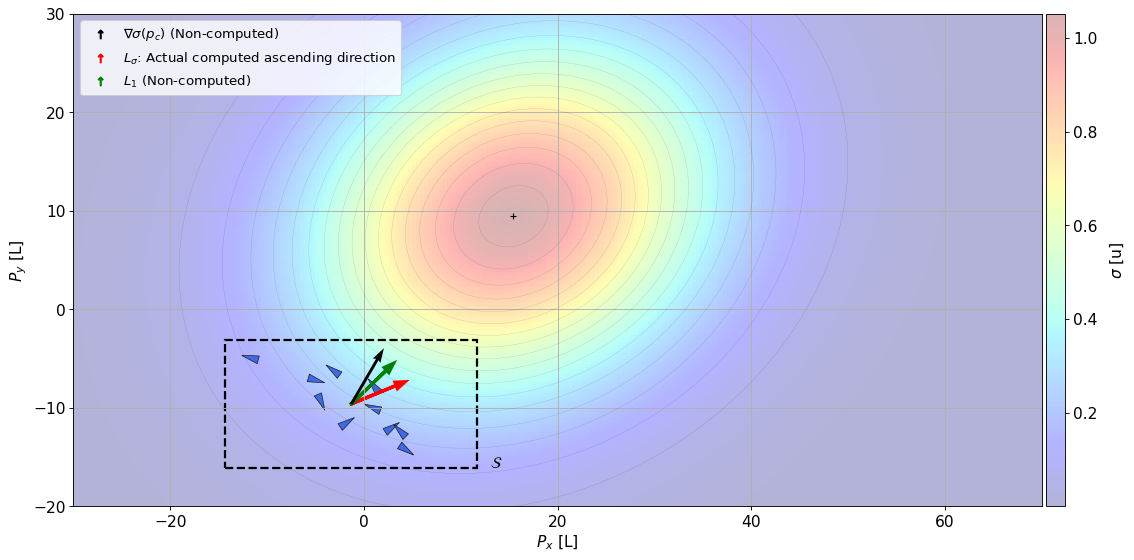
\includegraphics[trim={0 0cm 0 0cm}, clip, width=0.8\columnwidth]{./fig/lemma_1.png}
\caption{Para una formación genérica $x$ y señal gaussiana $\sigma$, se visualiza $\nabla\sigma(p_c)$, un posible conjunto $\mathcal{S}$, y el cómputo de $L_\sigma$ y $L_\sigma^1$. Resulta interesante visualizar que ninguno de estos vectores son paralelos. }
\label{fig: ss_lemma1}
\end{figure}

\newpage

Recordemos que $L^1_\sigma$ no es la aproximación de primer orden de $L_\sigma$ con respecto a $x_i$, sino que considera la aproximación de primer orden de $\sigma$. Teniendo esto en cuenta, el Lema \ref{rem: L1} conviene contrastarlo con (\ref{eq: Lsigma}), que como ya veremos únicamente es una dirección de ascenso cuando se impone cierta condición conservadora. No obstante, dicha condición se derivará teniendo en cuenta que $L^1_\sigma$ es siempre una dirección de ascenso. La idea del Lema \ref{le: l1}, motivó al autor de \cite{tfg_antonio} a analizar cómo de rápido diverge $L^1_\sigma$ de $L_\sigma$ en relación a $\|x\|$. 

\vspace{0.5cm}

\begin{lemma} \label{lem: ll1}
Para una señal $\sigma$, la divergencia entre $L^1_\sigma(p_c,x)$ y $L_\sigma(p_c,x)$ depende linealmente de $D := \max_{1 \le i \le N} | x_i |$ (es decir, la magnitud máxima de la distribución $x$). Es decir,

\begin{equation}
\|L_\sigma(p_c,x) - L^1_\sigma(p_c,x)\| \leq MD,\nonumber
\end{equation}

donde $M$ es el límite superior en \eqref{eq_grad_hess_bound}. Por lo tanto, $\lim_{D \to 0} \big( L_\sigma(p_c,x) - L^1_\sigma(p_c,x) \big) = 0$.
\end{lemma}

\begin{proof}
A partir de (\ref{eq: stay}), (\ref{eq: Lsigma}) y (\ref{eq: L1.1}), es fácil ver que
\begin{align}
    \|L_\sigma - L^1_\sigma\| &= \frac{1}{ND^2} \Bigg\|\sum_{i=1}^N \Big(\sigma(p_c + x_i) - \sigma(p_c) - \nabla\sigma(p_c)^Tx_i\Big)x_i\Bigg\| \nonumber \\
    &\leq \frac{1}{ND^2}\sum_{i=1}^N M||x_i||^3 \leq MD. \nonumber
\end{align}
\end{proof}

% ---

De hecho, si $D$ es lo suficientemente pequeño, entonces es seguro que $L_\sigma$ es una dirección de ascenso, al igual que $L_\sigma^1$. Sin embargo, ¿qué se considera como \textbf{pequeño} para señales y despliegues genéricos? Definamos $E := L_\sigma - L_\sigma^1$, de modo que

\begin{equation}
\nabla \sigma(p_c)^T L_\sigma = \nabla \sigma(p_c)^T (L_\sigma^1 + E),
\end{equation}

y consideremos un conjunto compacto $\mathcal{S} \subset \mathbb{R}^m$ con $p_\sigma \notin \mathcal{S}$. Por la definición de $\sigma$ y su gradiente acotado, sabemos que $\nabla \sigma(p_c)^T L_\sigma^1$ tiene un mínimo $F_\mathcal{S}(x)$ que depende del despliegue elegido $x$ y es positivo si $x$ no es degenerado, para todo $p_c \in \mathcal{S}$. Por lo tanto, tenemos $\nabla \sigma(p_c)^T L_\sigma \geq F_\mathcal{S}(x) - K_\mathcal{S}^+ M_\mathcal{S} D$, donde $K_\mathcal{S}^+$ y $M_\mathcal{S}$ son las normas máximas del gradiente y Hessiano de la señal en $\mathcal{S}$, respectivamente; por lo tanto, si

\begin{equation}
\label{eq: xiD}
F_\mathcal{S}(x) - K_\mathcal{S}^+ M_\mathcal{S} D > 0,
\end{equation}

entonces $L_\sigma$ es una dirección de ascenso en $\mathcal{S}$. Encontrar el mínimo $F_\mathcal{S}(x)$ numéricamente puede ser una tarea ardua, pero podemos acotarlo de manera conservadora utilizando el siguiente resultado de \cite{tfg_antonio}.

\newpage

\begin{lemma}
\label{lem: gradD}
Si $x$ no es degenerado, entonces existe $C(x) > 0$, que solo depende del despliegue del conjunto de robots, tal que
\begin{equation}
\frac{1}{C(x)}||\nabla\sigma(p_c)||^2 \leq L^1_\sigma(p_c, x)^T\nabla\sigma(p_c) \leq C(x) ||\nabla\sigma(p_c)||^2. \nonumber
\end{equation}
\end{lemma}

\begin{proof}
En primer lugar, vemos que el caso trivial $\nabla\sigma(p_c) = 0$ satisface la afirmación. En cualquier otro caso, sabemos por el Lema \ref{le: l1} que $\nabla\sigma(p_c)^TL^1_\sigma(p_c, x) = \frac{1}{ND^2}\sum_{i=1}^N |\nabla\sigma(p_c)^Tx_i|^2 = \frac{1}{ND^2} \nabla\sigma(p_c)^T P(x) \nabla\sigma(p_c) > 0$ para alguna matriz definida positiva $P(x) = \sum_{i=1}^N x_ix_i^T$ ya que $x$ no es degenerado. Por lo tanto,

\begin{equation}
\frac{\lambda_{\text{min}}{P(x)}}{ND^2} || \nabla \sigma ||^2 \le \nabla\sigma^T L^1_\sigma \le \frac{\lambda_{\text{max}}{P(x)}}{ND^2} || \nabla \sigma ||^2, \nonumber
\end{equation}

donde $\lambda_{\text{{min,max}}}{P(x)}$ son los valores propios mínimo y máximo de $P(x)$. Elegimos $C(x) = \max{ \frac{\lambda_{\text{max}}{P(x)}}{ND^2}, \frac{ND^2}{\lambda_{\text{min}}{P(x)}} }$, y solo depende del despliegue $x$.\\

\end{proof}

Ahora ya estamos listos para establecer una condición más fácil de verificar que (\ref{eq: xiD}), utilizando el primer resultado original que presentamos en esta metodología:

\vspace{0.2cm}

\begin{prop} \label{pro: S}
Sea $\mathcal{S}$ un conjunto compacto con $p_\sigma \notin \mathcal{S}$. Entonces, si
\begin{equation}
\lambda_{\text{min}}\{P(x)\} K^-_\mathcal{S} - NM_\mathcal{S}D^3 > 0, \nonumber
\end{equation}
donde $K^-_\mathcal{S}$ es la norma mínima del gradiente en el conjunto compacto $\mathcal{S}$, entonces $L_\sigma(p_c, x)$ es una dirección de ascenso en $p_c \in \mathcal{S}$.
\end{prop}
\begin{proof}
El Lema \ref{lem: gradD} acota inferiormente $F_\mathcal{S}(x)$ en (\ref{eq: xiD}); por lo tanto, tenemos que
    
\begin{align}
\nabla\sigma(p_c)^TL_\sigma &= \nabla\sigma(p_c)^TL^1_\sigma + \nabla\sigma(p_c)^TE \nonumber \\
&= \frac{1}{ND^2}\nabla\sigma(p_c)^TP(x)\nabla\sigma(p_c) + \nabla\sigma(p_c)^TE \nonumber \\
&\geq \frac{\lambda_{\text{min}}\{P(x)\}}{ND^2} ||\nabla\sigma(p_c)||^2 + \nabla\sigma(p_c)^TE.
\nonumber
\end{align}

Por lo tanto, para garantizar que $L_\sigma(p_c)$ sea una dirección de ascenso en $p_c\in\mathcal{S}$, es suficiente satisfacer $\frac{\lambda_{\text{min}}\{P(x)\}}{ND^2} |\nabla\sigma(p_c)|^2 + \nabla\sigma(p_c)^E > 0$. Es decir, si

\newpage

\begin{align}
\nabla\sigma(p_c)^TL_\sigma &= \frac{\lambda_{\text{min}}\{P(x)\}}{ND^2} ||\nabla\sigma(p_c)||^2 - ||\nabla\sigma(p_c)||M_\mathcal{S}D \nonumber \\
&= ||\nabla\sigma(p_c)||\left(\frac{\lambda_{\text{min}}\{P(x)\} ||\nabla\sigma(p_c)|| }{ND^2} - M_\mathcal{S}D \right) \nonumber \\
&\propto \lambda_{\text{min}}\{P(x)\} K^-_\mathcal{S} - NM_\mathcal{S}D^3 \; > \; 0, \nonumber
\end{align}

entonces $\nabla\sigma(p_c)^TL_\sigma > 0$; por lo tanto, se satisface la condición (\ref{eq: xiD}) y $L_\sigma(p_c)$ es una dirección de ascenso en $p_c\in\mathcal{S}$. \\
\end{proof}

En la Proposición \ref{pro: S}, la dependencia con $N$ es un poco engañosa. Recordemos que $P(x) = \sum_{i=1}^Nx_ix_i^T$, de modo que para algún $a\in\mathbb{R}^m$ no nulo, la expresión $a^T P(x) a > 0$ puede ser acotada inferiormente por ${\operatorname{min}}\{\lambda_\text{min}\{x_ix_i^T + x_jx_j^T\}\} \frac{1}{2}N||a||^2$, lo que haría desaparecer a $N$ de la condición. Podemos decir algo similar sobre la dependencia en $D$, ya que $P(x)$ incorpora $D^2$ debido a que consiste en los elementos $x_ix_i^T$; por lo tanto, la dependencia efectiva de la Proposición \ref{pro: S} en $D$ es lineal, no cúbica. Esta última observación no es sorprendente, ya que coincide con el resultado del Lema \ref{lem: ll1}.

Aunque la señal $\sigma$ sea desconocida, gracias a la Proposición \ref{pro: S}, siempre podemos diseñar $D$ en función de los escenarios esperados. Por ejemplo, supongamos la liberación de un contaminante; los científicos pueden estimar los valores de $M_\mathcal{S}$, $K_\mathcal{S}^+$ y $K_\mathcal{S}^-$ para los umbrales mínimos/máximos de contaminación en el \textbf{área de patrullaje} $\mathcal{S}$, donde el equipo de robots necesita reaccionar de manera confiable. También resulta interesante destacar que, al diseñar $L^1_\sigma$ de forma paralela al gradiente $\nabla\sigma(p_c)$, también se hace que el producto escalar $\nabla\sigma(p_c)^TL_\sigma > 0$ más robusto en relación a $D$.

Hasta ahora, nuestra metodología ha requerido de una topología en estrella, lo que significa que todo el conjunto de robots deja de funcionar si la unidad de cómputo que actúa como núcleo desaparece. Si bien seleccionar robots de respaldo podría ser una solución, un enfoque alternativo es distribuir los cálculos en una red arbitraria de subequipos dentro del enjambre de robots. Dicha red mejoraría la resiliencia del enjambre de robots, ya que los distintos subequipos podrían unirse o abandonar al enjambre sin afectar significativamente el rendimiento de la misión, al mismo tiempo que reduciría las necesidades en infraestructura de comunicación. Proponemos entonces una red arbitraria de equipos en una topología en estrella (ver \autoref{fig: pctilde}), donde la \textbf{dirección de ascenso común} $\tilde L_\sigma$ se logra mediante un algoritmo estándar de consenso \cite{olfati2004consensus}, es decir, las unidades de cómputo de los equipos vecinos compartirán sus direcciones de ascenso para alcanzar el consenso de que

\begin{equation} \label{l_sigma_tilde}
\tilde L_\sigma = \frac{1}{N_c}\sum^{N_c}_{k=1}L_{\sigma_k}(p_c^k, x^k).
\end{equation}

\newpage

\vspace{0.3cm}

\begin{figure}[!h]
    \centering
    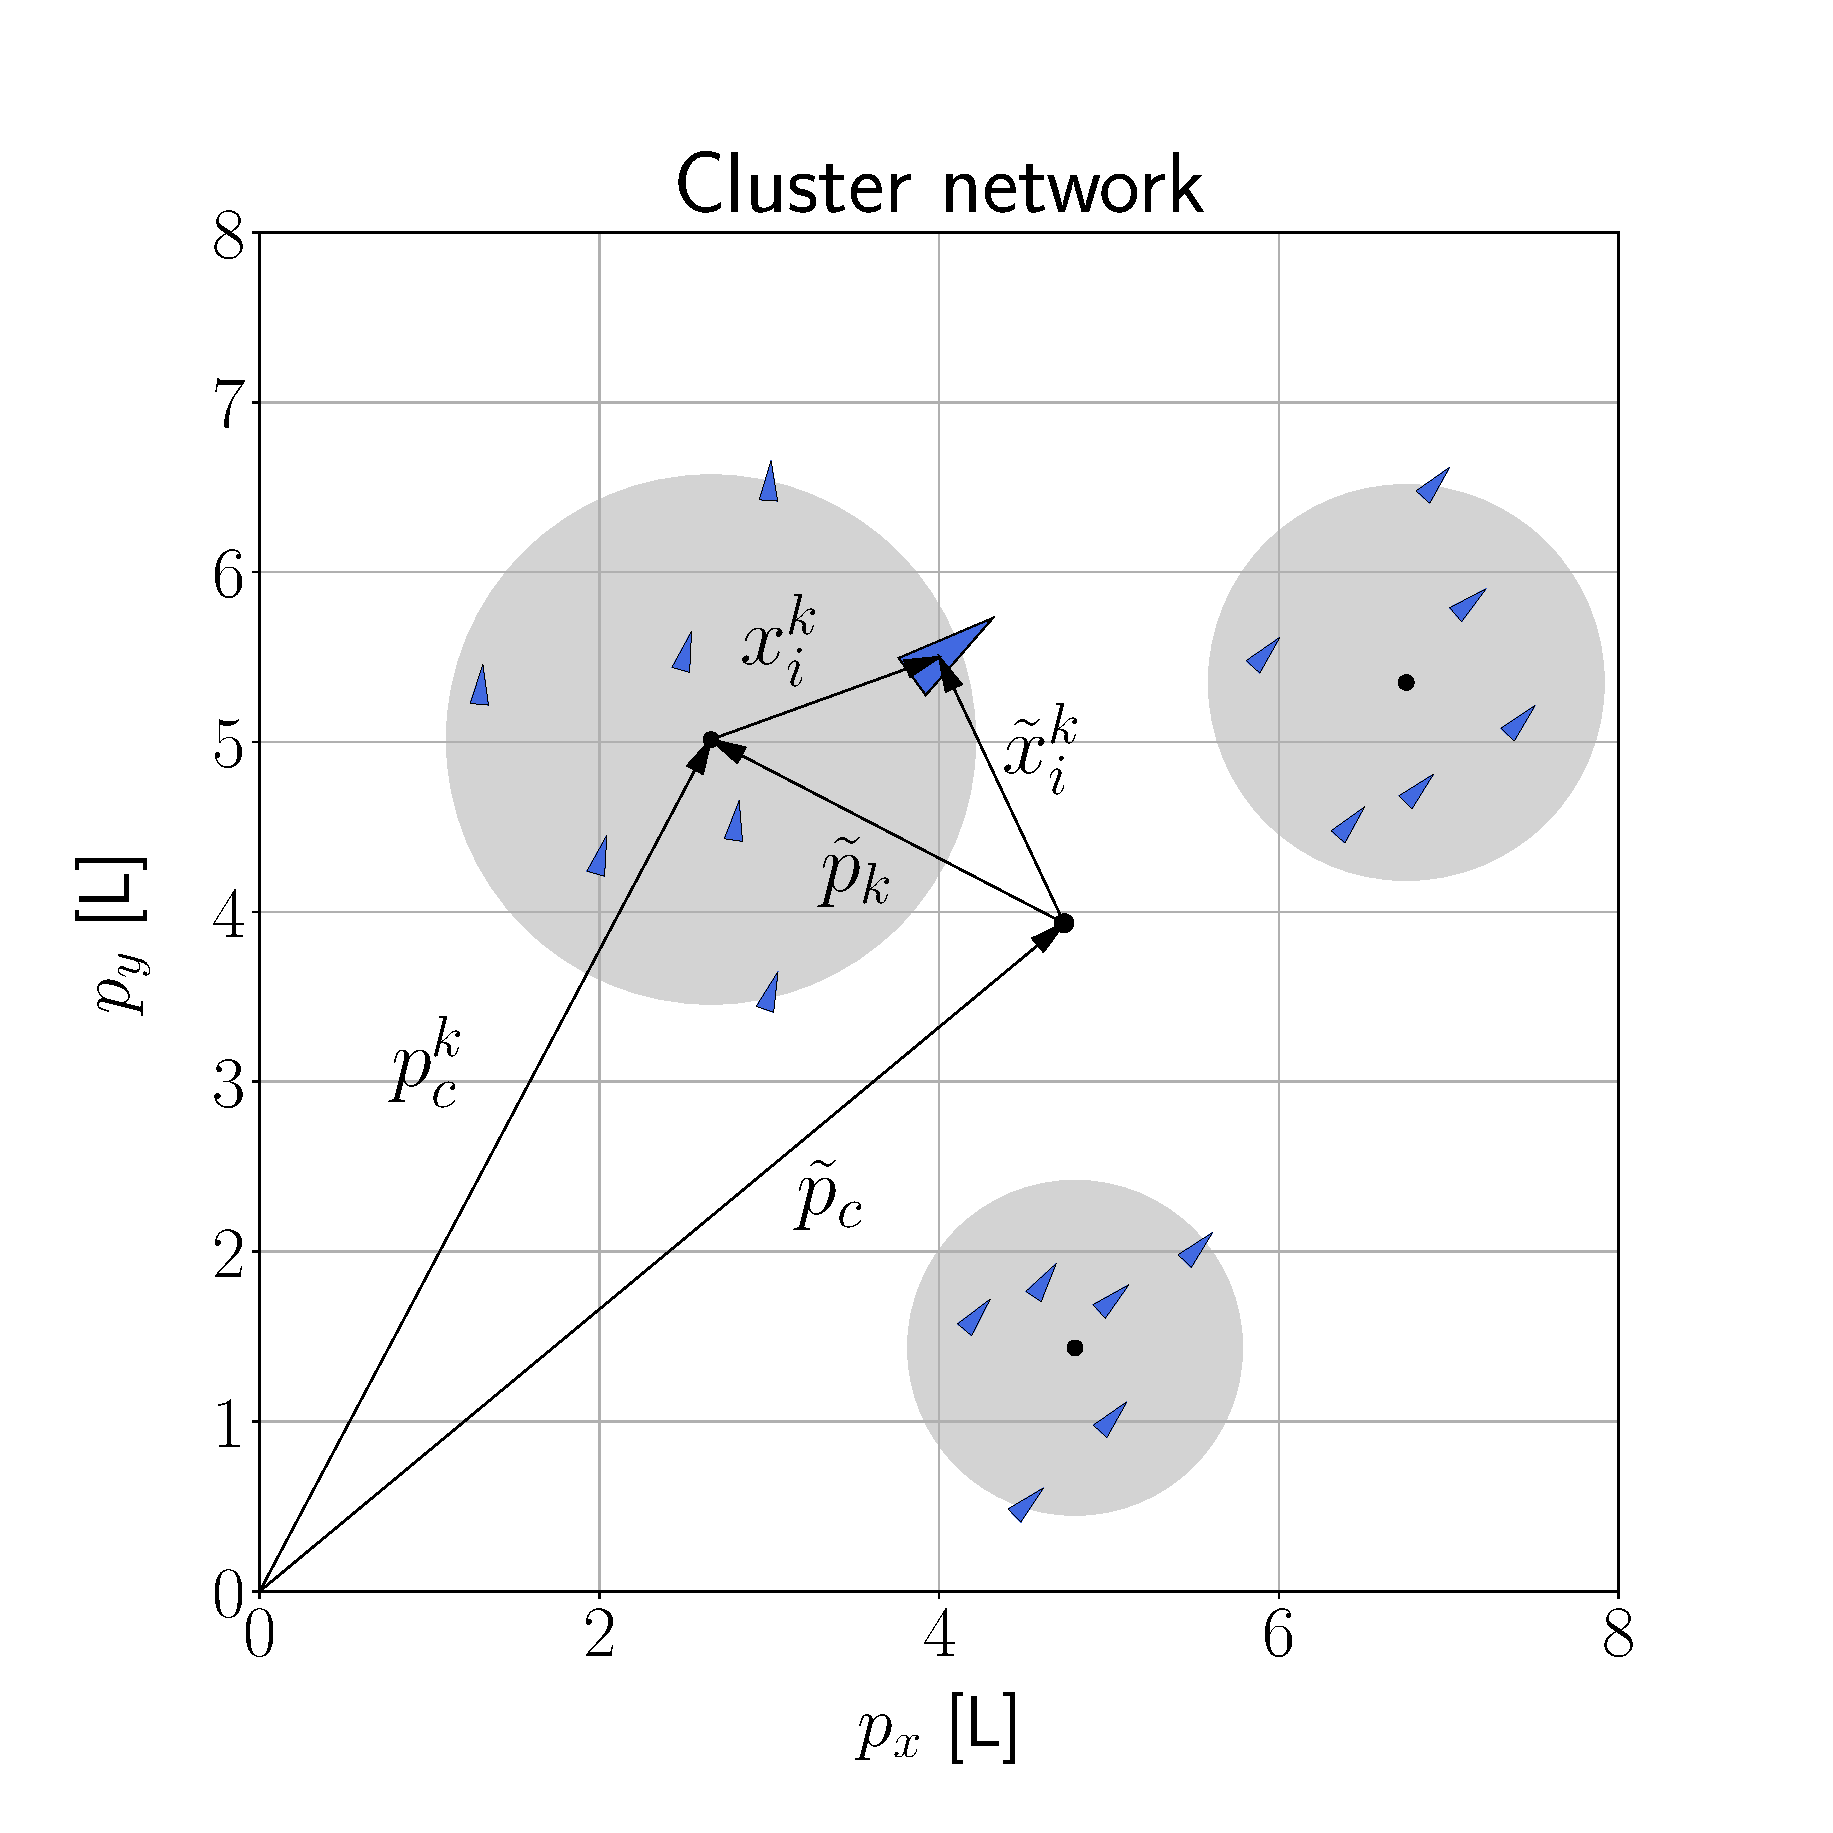
\includegraphics[trim={0 0 0 3.34cm}, clip, width=0.6\columnwidth]{./fig/pctilde.eps}
    \caption{En esta figura se visualiza toda la notación para un caso en el que tres equipos coordinados computan una dirección de ascenso común $\tilde L_\sigma$.}
    \label{fig: pctilde}
\end{figure}

La pregunta que nos hacemos ahora es si $\tilde L_\sigma$ es una dirección de ascenso en el centroide de centroides $\tilde p_c$. Dado que el sumatorio de productos escalares positivos siempre va a ser estrictamente mayor que cero, está claro que si $L_{\sigma_k}(p_c^k, x^k)$ es una dirección de ascenso en $\tilde p_c$ para todos los $k \in \{1,\dots,N_c\}$, entonces $\tilde L_\sigma$ también lo será (ver \autoref{fig: ss_col1}). Inicialmente, puede parecer un trabajo redundante, ya que si se encuentra una dirección de ascenso, el resto de los subequipos podrían adoptarla. Sin embargo, en la práctica, el algoritmo de consenso va a ofrecer una gran robustez, ya que elimina la necesidad de diseñar una lógica adicional para determinar qué $L_k(p_c^k, x^k)$ son admisibles en cada $p_c^k$, al tiempo que permite a los subequipos un modo seguro de fusionarse o salir de la red. Es interesante señalar que cualquier robot puede pertenecer a múltiples subequipos simultáneamente, lo que permite la superposición y mejora la resiliencia del enjambre de robots.

También conviene destacar que el algoritmo de consenso, donde todas las unidades de cómputo vecinas comparten sus $L_{\sigma_k}(p_c^k, x^k)$, converge rápidamente al valor común de forma exponencial. Esta es otra característica importante en la práctica, ya que $L_{\sigma_k}(p_c(t)^k, x^k)$ varía con el tiempo y la velocidad de los robots determinará el ancho de banda para ejecutar el algoritmo de consenso. En conclusión, la convergencia exponencial a $L_{\sigma_k}$ aliviará esta necesidad de ancho de banda. 

A continuación, mostraremos cómo garantizar que $L_{\sigma_k}(p_c^k, x^k)$ sea una dirección de ascenso en $\tilde p_c$. Sabemos que si el $k$-ésimo clúster elige su $D$ (o $D_k$) de acuerdo con la Proposición \ref{pro: S}, entonces hay un margen para variar $p_c^k$ de manera que $L_{\sigma_k}$ sea una dirección de ascenso en $\tilde p_c = p_c^k + \tilde p_k$. Veamos cómo hacerlo.

Consideremos la siguiente expansión en serie de Taylor entorno a $p_c^k$:

\begin{equation}
\nabla\sigma(p_c^k + \tilde p_c^k) = \nabla\sigma(p_c^k) + H(p_c^k)\tilde p_c^k + \mathcal{O}(\|\tilde p_c^k\|^2), \nonumber
\end{equation}

\newpage

y definamos $\tilde E := \nabla\sigma(p_c^k + \tilde p_c^k) - \nabla\sigma(p_c^k)$. Entonces tenemos que

\begin{equation}
\| \tilde E \| \leq M \|\tilde p_c^k \|. \nonumber
\end{equation}

Al igual que en la demostración de la Proposición \ref{pro: S}, debemos asegurarnos de que el producto escalar $L_{\sigma_k}^T\nabla\sigma(p_c^k + \tilde p_c^k) > 0$ para que $L_{\sigma_k}$ sea una dirección de ascenso en $\tilde p_c$. Esto es equivalente a verificar si

\begin{equation}
L_{\sigma_k}^T\nabla\sigma(p_c^k + \tilde p_c^k) = L_{\sigma_k}^T\nabla\sigma(p_c^k) + L_{\sigma_k}^T\tilde E > 0, \nonumber
\end{equation}

lo que nos lleva a presentar nuestro segundo resultado original para esta metodología, un corolario de la Proposición \ref{pro: S}.

\begin{coroll} \label{cor: clus}
Dado un enjambre de robots formado por $N_c$ (sub)equipos, tendremos que $\tilde L_\sigma$ es una dirección de ascenso en $\tilde p_c \in \mathcal{S}$ si $\forall k\in\{1,\dots,N_c\}$
\begin{equation}
\lambda_{\text{min}}\{P(x^k)\} K^-_\mathcal{S} - M_\mathcal{S}(N_kD_k^3 + \|\tilde p^k_c\|)> 0. \nonumber
\end{equation}
\end{coroll}

Cuando contemos con más de una unidad de cómputo en un mismo enjambre, el Corolario \ref{cor: clus} nos dice que será más sencillo satisfacer la condición para que $\tilde L_{\sigma}$ sea dirección de ascenso cuanto menor sea $D_k$ y la distancia de los equipos al centroide de centroides $\|\tilde p_c^k\|$. Es decir, siempre será conveniente minimizar el tamaño de los equipos y la distancia entre ellos. Véase que la dependencia de $N$ también es un poco engañosa en esta condición, pues cuanto mayor sea el número de agentes del equipo $k$, menor será el valor de $\|\tilde p_c^k\|$ según la definición de centroide.

\vspace{0.2cm}

\begin{figure}[!h]
\centering
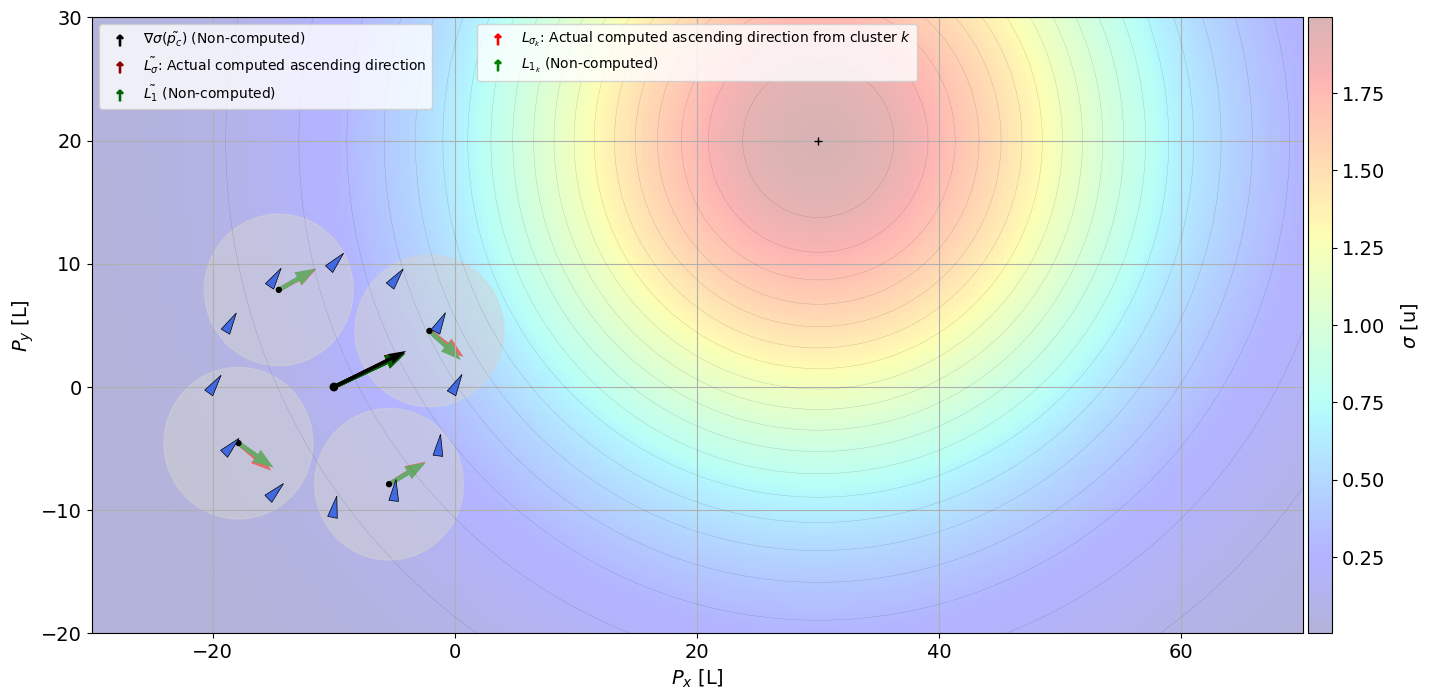
\includegraphics[trim={0 0cm 0 0cm}, clip, width=1\columnwidth]{./fig/col_1.png}
\caption{En esta figura tenemos a un enjambre formado por cuatro (sub)equipos. La unidad de cómputo de cada uno de los equipos calcula su $L_{\sigma_k}$ y la comparte con el resto para calcular de forma distribuida $\tilde L_{\sigma_k}$.}
\label{fig: ss_col1}
\end{figure}

\newpage

Concluimos esta subsección mencionando que el Corolario \ref{cor: clus} también se puede emplear para diseñar la implementación de diferentes equipos que patrullan un mismo área. Si están en riesgo de colisión, podrán fusionarse con garantías y tener una dirección de ascenso común para el nuevo centroide creado.


% Análisis de observabilidad y sensibilidad
%%%%%%%%%%%%%%%%%%%%%%%%%%%%%%%%%%%%%%%%%%%%%%%%%%%%%%%%%%%

\subsubsection{Análisis de observabilidad y sensibilidad}

El análisis de cómo ciertos despliegues $x$ generan una dirección $L^1_{\sigma}$ paralela al gradiente $\nabla \sigma(p_c)$, y la sensibilidad de dicho paralelismo ante modificaciones en el despliegue, es crucial para obtener enjambres de robots más resilientes en la resolución del problema de \textit{souce-seeking}; por ejemplo, si consideramos desplazamientos erróneos de los robots o transformaciones de la formación a lo largo de la misión. Al fin y al cabo, las magnitudes de $L^1_{\sigma}$ y $L_\sigma$ no son tan importantes, especialmente si queremos mantener independiente la velocidad de los robots de dichas magnitudes, es decir, simplemente rastrear $\frac{L_\sigma}{|L_\sigma|}$. Además, veremos que para algunos despliegues tenemos que $L^1_{\sigma} = L_\sigma$ cuando aproximamos la señal $\sigma(p_c)$ hasta segundo orden alrededor de $p_c$.

Con el fin de ser ilustrativos, comenzaremos el análisis proponiendo el caso discreto de cuatro robots formando un rectángulo ($x^{\text{4rct}}$ en la \autoref{fig: 4rect}), luego un polígono regular, y aplicamos algunas transformaciones afines para comprobar la sensibilidad de las direcciones de ascenso. Posteriormente, desplegamos \emph{un enjambre de robots} dentro de una forma siguiendo una distribución de densidad ($x^{\text{rct}}$ en la \autoref{fig: 4rect}), es decir, consideramos $N\to\infty$, y mostramos condiciones de simetría suficientes para que $L^1_{\sigma}$ sea paralelo al gradiente.

\vspace{0.4cm}

\begin{figure}[!h]
\centering
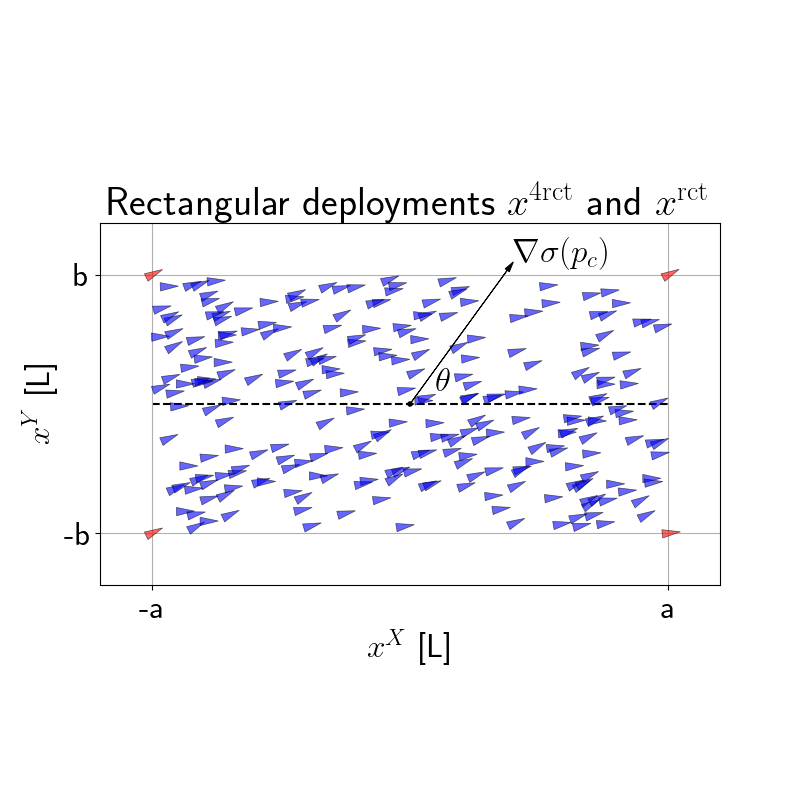
\includegraphics[trim={0 3.4cm 0 5.67cm}, clip, width=0.8\columnwidth]{./fig/4rect.png}
\caption{La formación rectangular de 4 robots $x^\text{4rct}$ se encuentra en las esquinas del rectángulo en color rojo. Los 250 robots en color azul pertenecen a la formación $x^\text{rct}$ y están distribuidos uniformemente dentro del rectángulo. El gradiente $\nabla\sigma(p_c)$ es arbitrario y forma un ángulo $\theta$ con el eje horizontal de la formación rectangular.}
\label{fig: 4rect}
\end{figure}

\newpage

Consideremos cuatro robots en las esquinas de un rectángulo y, sin pérdida de generalidad, supongamos que el lado largo del rectángulo es paralelo al eje horizontal, de modo que el gradiente $\nabla\sigma(p_c) = |\nabla\sigma(p_c)| \left[\begin{smallmatrix}\cos(\theta) & \sin(\theta) \end{smallmatrix}\right]^T$ tiene una norma y un ángulo arbitrarios (ver Figura \ref{fig: 4rect}). Entonces, la dirección de ascenso $L^1_{\sigma}$ se puede escribir como

\begin{equation} \label{eq: L1theta}
L^1_\sigma(p_c, x) = \frac{\|\nabla\sigma(p_c)\|}{ND^2} \sum_{i=1}^N \left(\begin{bmatrix}\cos(\theta) & \sin(\theta) \end{bmatrix} \begin{bmatrix}x_i^X \\ x_i^Y \end{bmatrix}\right)\begin{bmatrix}x_i^X \\ x_i^Y \end{bmatrix},
\end{equation}

donde los superíndices $X$ e $Y$ denotan las coordenadas horizontales y verticales de $x_i$ con respecto a un sistema de referencia arbitrario, como se muestra en la Figura \ref{fig: 4rect}. Por lo tanto, para los cuatro robots en las esquinas del rectángulo con despliegue $x^{4\text{rct}}$ tenemos que

\begin{align}
&L^1_\sigma(p_c, x^{4\text{rct}}) = \frac{\|\nabla\sigma(p_c)\|}{4(a^2+b^2)}\bigg(\big(a\cos(\theta)+b\sin(\theta)\big)\begin{bmatrix}a\\b \end{bmatrix} + \nonumber \\ 
&+\big(-a\cos(\theta)+b\sin(\theta)\big)\begin{bmatrix}-a\\b \end{bmatrix}
+ \big(-a\cos(\theta)-b\sin(\theta)\big)\begin{bmatrix}-a\\-b \end{bmatrix} + \nonumber \\
&+ \big(a\cos(\theta)-b\sin(\theta)\big)\begin{bmatrix}a\\-b \end{bmatrix} \bigg) = \frac{\|\nabla\sigma(p_c)\|}{(a^2 + b^2)}\begin{bmatrix}a^2\cos(\theta)\\b^2 \sin(\theta)\end{bmatrix}, \nonumber %\label{eq: l1sq4}
\end{align}

donde podemos observar que para el cuadrado ($a=b$), tenemos que $L^1_\sigma(p_c, x^{4\text{rct}}) = \frac{1}{2}\nabla\sigma(p_c)$. Finalmente, si $a$ o $b$ es igual a cero (pero no ambos) para la formación rectangular $x^{4\text{rct}}$, en $L^1_\sigma(p_c, x^{4\text{rct}})$ únicamente se observará la proyección de $\nabla\sigma(p_c)$ en la línea descrita por la formación $x$ degenerada. No obstante, hay que tener en cuenta que en este caso los robots colapsarían por parejas en dos puntos coincidentes. Esta situación indeseable es la que nos motivó para llegar al siguiente resultado.

\vspace{0.2cm}

\begin{prop} [Observabilidad con formaciones en cruz]
\label{prop: cross}
Consideremos dos formaciones degeneradas en 2D (segmentos) y perpendiculares con longitudes iguales; es decir, $x^\parallel$ y $x^-$ con $N_\parallel$ y $N_-$ números de robots, que están distribuidos simétricamente alrededor del centroide, de modo que ambos despliegues comparten su centroide. Considerando uno de los segmentos, su robot más lejano $1$ se encontrará a una distancia $a_1 \in \mathbb{R}$, mientras que el resto de sus robots $i\in\{1, \dots, \frac{N}{2}\}$ a distancias $0 \leq a_{i+1} < a_i$ tal que $\sum_{i=2}^{\frac{N}{2}}a_i^2 = \frac{N}{4}a_1^2$. Entonces, $\lim_{N_\parallel\to\infty} L^1_\sigma(p_c, x^\parallel) + \lim_{N_-\to\infty} L^1_\sigma(p_c, x^-) = \frac{1}{2}\nabla\sigma(p_c)$.
\end{prop}

\begin{proof}
En primer lugar, observemos que un robot en $x_i = 0$ no contribuye en absoluto al cómputo de $L_{\sigma}$; por lo tanto, dado que requerimos simetría reflectante alrededor de $x = 0$, podemos suponer que $N_\parallel$ y $N_-$ son pares para que sus mitades también sean números enteros. Además, dado que los dos segmentos tienen la misma longitud, podremos asumir que $a_{1_\parallel} = a_{1_-} = a_1$. Entonces, de acuerdo con (\ref{eq: L1.1}), tenemos que

\begin{equation}
L^1_\sigma(p_c, x^\parallel) = \frac{\|\nabla\sigma(p_c)\|\cos(\theta)}{N_\parallel a_1^2} 2\sum_{i=1}^{\frac{N_\parallel}{2}}\begin{bmatrix}a_i^2 \\ 0 \end{bmatrix}.
\nonumber
\end{equation}

Aplicando la condición $\sum_{i=2}^{\frac{N}{2}}a_i^2 = \frac{N}{4}a_1^2$ del enunciado, que se puede verificar como factible para una serie geométrica $a_{i+1} = \alpha a_i, \, i \in \{1, \dots, (\frac{N_\parallel}{2}-1)\}$ para algún $0 < \alpha < 1$, y $a_{\frac{N_\parallel}{2}} = -\left(\sum_{i=2}^{\frac{N}{2}-1}a_i^2 -\frac{N}{4}\right) < a_1^2$, tenemos que

\begin{align}
L^1_\sigma(p_c, x^\parallel) &= \frac{2\|\nabla\sigma(p_c)\|\cos(\theta)}{N_\parallel a_1^2} \begin{bmatrix}a_1^2 + \frac{N_\parallel}{4}a_1^2 \\ 0\end{bmatrix} \nonumber \\
&= \frac{1}{2}\|\nabla\sigma(p_c)\|\cos(\theta) \begin{bmatrix}\frac{4 + N_\parallel}{N_\parallel} \\ 0\end{bmatrix}. \nonumber
\end{align}

De manera similar, podemos obtener que 

\begin{align}
L^1_\sigma(p_c, x^-) = \frac{1}{2}\|\nabla\sigma(p_c)\|\sin(\theta) \begin{bmatrix}0 \\ \frac{4 + N_-}{N_-}\end{bmatrix}. \nonumber
\end{align}

Por lo tanto, si las dos unidades de cómputo combinan sus resultados, tendremos que 

$$
\lim_{N_\parallel\to\infty} L^1_\sigma(p_c, x^\parallel) + \lim_{N_-\to\infty} L^1_\sigma(p_c, x^-) = \frac{1}{2}\nabla\sigma(p_c).
$$
\end{proof}

\begin{figure}[!h]
\centering
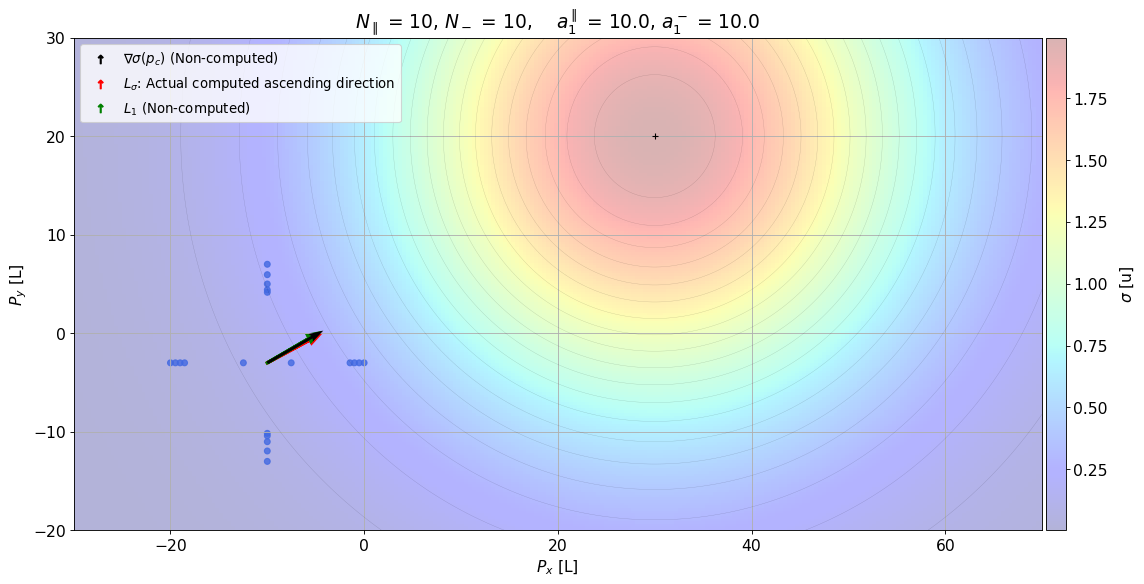
\includegraphics[trim={0 0 0 0}, clip, width=1\columnwidth]{./fig/ss_prop2.png}
\caption{Para una señal gaussiana $\sigma$ y una formación $x^{\text{cross}}$, como la que se introduce en la Proposición \ref{prop: cross}, en esta figura se muestra el cómputo de $L^1_\sigma(p_c, x^{\text{cross}})$ y $L_\sigma(p_c, x^{\text{cross}})$. Dado que $N_\parallel = N_-$ y $a_{1_\parallel} = a_{1_-}$, podemos comprobar que $L^1_\sigma(p_c, x^{\text{cross}})$ es paralelo al gradiente.}
\label{fig: ss_prop2}
\end{figure}  

\newpage

La demostración de la Proposición \ref{prop: cross} nos permite intuir que si $N_\parallel = N_-$, entonces la dirección de ascenso resultante es paralela al gradiente $\nabla\sigma(p_c)$ (ver \autoref{fig: ss_prop2}), un resultado que también puede obtener en 3D para una distribución equivalente. Por supuesto, el procedimiento de diseño se puede modificar para que, cuando $N_\parallel \neq N_-$ y $a_{1_\parallel} \neq a_{1_-}$, el resultado sea el mismo que en la Proposición \ref{prop: cross}. La serie geométrica propuesta para la distribución de los robots es solo una sugerencia. Dado que lo que importa es la dirección de $L_\sigma^1$, la suma $\sum_{i=2}^{\frac{N}{2}}a_i^2$ siempre podrá ser ajustada en cada segmento de forma independiente para compensar aquellos casos en los que $N_\parallel \neq N_-$ o $a_{1_\parallel} \neq a_{1_-}$.

También es bastante directo comprobar que el grupo de 3 robots $x^{3\text{tri}}$ formando un triángulo equilátero con centroide en $p_c$ calcula $L^1_\sigma(p_c, x^{3\text{tri}})$ de forma paralela al gradiente $\nabla\sigma(p_c)$. En general, cualquier formación que forme un \textbf{polígono regular} tendrá su $L^1_\sigma(p_c, x^{N\text{poly}})$ paralelo al gradiente $\nabla\sigma(p_c)$. Este resultado ya se ha descubierto en \cite{brinon2015distributed}, donde los robots están distribuidos de manera equitativa en una circunferencia, es decir, describen un polígono regular. Sin embargo, ¿cuál es la sensibilidad de $L^1_\sigma(p_c, x^{N\text{poly}})$ en relación a posibles desplazamientos incorrectos o ligeras modificaciones en la formación regular? 


Aunque ya hemos demostrado en el Lema \ref{le: l1} que, independientemente de $x$, $L^1_\sigma(p_c, x)$ es siempre una dirección de ascenso, proporcionaremos más detalles al respecto, estudiando lo que sucede para distintas formaciones. Aunque el enjambre de robots calcula $L_\sigma$ en lugar de $L^1_\sigma$, este análisis es relevante porque, cuanto más paralelo sea $L^1_\sigma$ al gradiente $\nabla\sigma$, más robusta será la condición de ascenso $L_\sigma(p_c, x)^T\nabla\sigma(p_c) > 0$. 

En primer lugar, formalizaremos un resultado técnico que ya introducimos en la Observación \ref{rem: L1}, pues será necesario más adelante.

\begin{lemma}[Proporcionalidad con polígonos regulares] \label{le: 4}
Consideremos la distribución $x^{N\text{poly}}$ (o $x^{\text{3D-Npoly}}$ ) de $N$ robots formando un polígono regular (poliedro), y $b\in\mathbb{R}^m$, entonces

\begin{equation}
\sum_{i=1}^N \left(b^Tx_i\right)x_i \propto b. \nonumber
\end{equation}

\end{lemma}

\begin{proof}
Partimos del echo de que

\begin{equation}
\sum_{i=1}^N \left(b^T x_i\right)x_i = \sum_{i=1}^N(x_ix_i^T)b. \nonumber
\end{equation}

Para que esta expresión sea proporcional a $b$, es necesario que todos los elementos diagonales de la matriz semidefinida positiva $P = \sum_{i=1}^N(x_ix_i^T)$ sean iguales y que los elementos no diagonales sean nulos. Dado que todas las distribuciones consideradas se encuentran en la esfera $m$-dimensional, entonces todas las normas $||x_i||$ son iguales. Además, todos los ángulos diedros de las distribuciones consideradas son iguales, por lo que podemos encontrar ejes XYZ donde el conjunto de todas las proyecciones de los vértices $x_i$ en los planos XY, XZ e YZ exhibe una simetría par; por lo tanto, $\sum_i^N (x_i^X)^2 = \sum_i^N (x_i^Y)^2 = \sum_i^N (x_i^Z)^2$. Finalmente, un polígono regular tiene simetría de reflexión para un eje XY; por lo tanto, $\sum_i^N (x_i^X)(x_i^Y) = 0$. Esto también es cierto para un poliedro regular en los mismos planos XY, XZ e YZ.\\
\end{proof}

\newpage

\begin{figure}[!h]
\centering
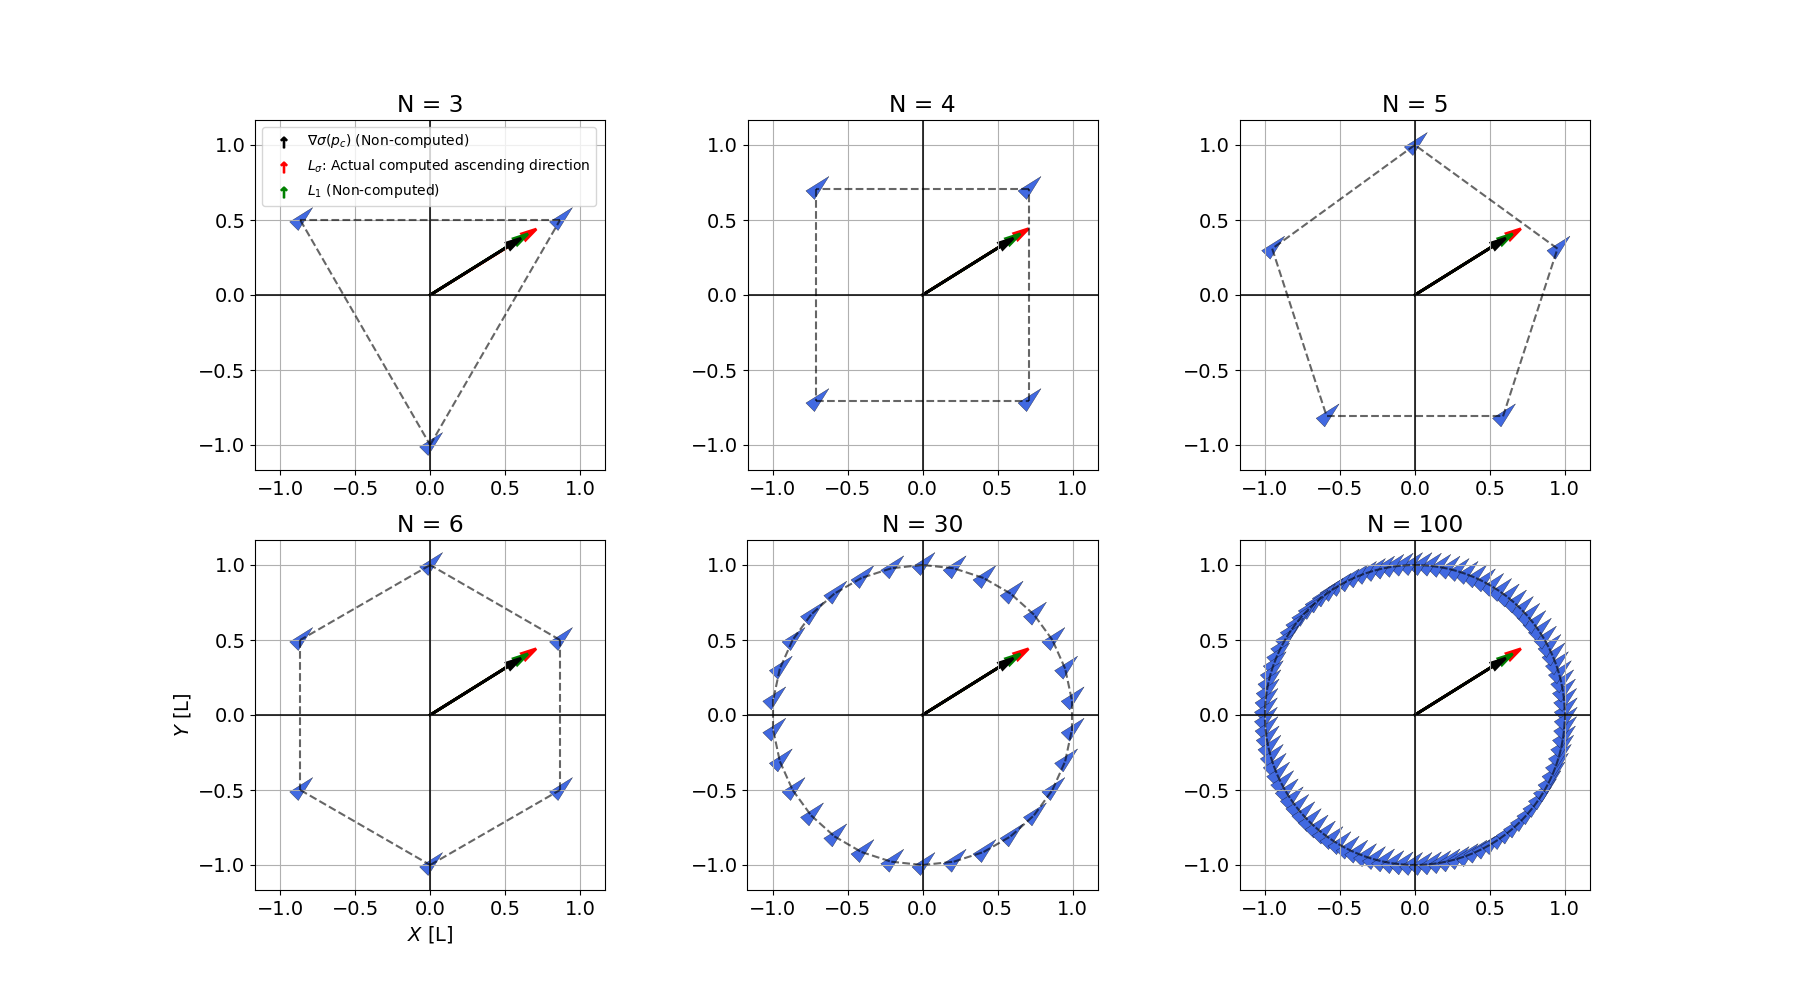
\includegraphics[trim={0 0 0 0}, clip, width=1\columnwidth]{./fig/lemma4.png}
\caption{En esta figura se muestra el cómputo de $L^1_\sigma(p_c, x^{N\text{poly}})$ y $L_\sigma(p_c, x^{N\text{poly}})$ para distintos valores de $N$. En todos los casos, se puede observar que $L^1_\sigma(p_c, x^{N\text{poly}})$ es paralelo al gradiente.}
\label{fig: ss_lemma4}
\end{figure}  

Para polígonos regulares en 2D, si alineamos el primer vértice con la línea horizontal de uno de los ejes de simetría y normalizamos la distancia de dicho vértice al centroide a $1$, entonces la suma de los cuadrados de todas las componentes $X$ de los vértices es $\sum_{i=1}^N (x_i^X)^2 = \sum_{i=0}^{N-1} \cos^2(\frac{i2\pi}{N})$, y debido a la simetría del polígono regular, la misma igualdad se cumple para $\sum_{i=1}^{N} (x_i^Y)^2$.

% ---

Ahora es fácil ver que $L^1_\sigma(p_c, x^{N\text{poly}}) \propto \left[\begin{smallmatrix}\cos\theta & \sin\theta \end{smallmatrix}\right]^T$, es decir, es paralelo al gradiente $\nabla\sigma(p_c)$ (ver \autoref{fig: ss_lemma4}), y para poliedros regulares $L^1_\sigma(p_c, x^{\text{3D-Npoly}}) \propto \left[\begin{smallmatrix}\sin\theta \cos\varphi & \sin\theta \sin\varphi & \cos\theta \end{smallmatrix}\right]^T$ con $\theta$ y $\varphi$ siendo la inclinación y azimut del gradiente en coordenadas esféricas, con origen en el centroide del poliedro regular 3D. 

De hecho, no necesitamos robots en todos los vértices del poliedro regular, sino solo un subconjunto. Por ejemplo, tomemos dos caras paralelas de un cubo; desde la primera, nos enfocamos en una diagonal y seleccionamos dos robots opuestos; desde la segunda cara, seleccionamos los robots en la otra diagonal perpendicular, entonces tendremos que $\sum_{i=1}^4 \left(b^Tx_i\right)x_i \propto b, b\in\mathbb{R}^3$ para los cuatro robots en esos vértices específicos de un cubo. Por lo tanto, estos cuatro robots son suficientes para calcular un $L^1_\sigma(p_c, x^{\text{4robots-cube}})$ paralelo al gradiente 3D $\nabla\sigma(p_c)$. En 2D, necesitaremos al menos tres robots formando un triángulo equilátero. El resultado presentado aquí en 3D también coincide con el trabajo presentado en \cite{brinon2019multirobot}; sin embargo, hemos llegado a la misma conclusión sin la necesidad de un uso intensivo de la trigonometría. De hecho, incluso podríamos extender los resultados presentados a $m>3$ dimensiones.

A continuación, analizaremos la sensibilidad de $L^1_\sigma(p_c, x^{N\text{poly}})$ \footnote{Para una notación más clara y concisa, no indicamos explícitamente 
 si el polígono regular es 2D o 3D, ambos casos los denotaremos como  $x^{N\text{poly}}$.} cuando la forma de la distribución está bajo una \textbf{transformación afín}; por ejemplo, escalado, rotación y cizalla, que podrían ser necesarias para explorar de forma efectiva un entorno desconocido para los robots. 
 
 En primer lugar, conviene apreciar que dicha transformación afín se puede aplicar formalmente con $(I_N \otimes A)x^{N\text{poly}}$, donde $A\in\mathbb{R}^{m\times m}$ es el operador lineal para la transformación. Dicho operador, siempre se podrá descomponer como un escalado y una rotación aplicando la descomposición en valores singulares (SVD, \textit{singular value decomposition}) $A = U\Sigma V^T$. La matriz $V$, que codifica las rotaciones, ya veremos que será irrelevante, pues $L^1_\sigma(p_c, x^{N\text{poly}})$ es paralelo al gradiente en $p_c$ para cualquier rotación de la distribución (ver \autoref{fig: ss_prop3}), tal y como se muestra en la siguiente proposición. 

\vspace{0.2cm}
 
\begin{prop}[Invarianza ante rotaciones]
\label{pro: RL1}
$L^1_\sigma(p_c, x^{N\text{poly}})$ es invariante para todas las distribuciones $(I_N \otimes R)x^{N\text{poly}}$ con $R\in$ SO$(m)$ siendo una matriz de rotación.
\end{prop}
\begin{proof}
En lo siguiente, definimos $r\in\mathbb{R}^m$ como el vector unitario que marca la dirección del gradiente $\nabla\sigma(p_c)$, y definimos su rotación por $R^T$ como $\tilde r = R^Tr$. Luego, aplicando la transformación $R$ a cada $x_i$, tenemos que

\begin{align}
L^1_\sigma(p_c,(I_N \otimes R) x^{N\text{poly}}) &= \frac{|\nabla\sigma(p_c)|}{ND^2}\sum_{i=1}^N \Big(r^T Rx_i\Big)Rx_i = \frac{|\nabla\sigma(p_c)|}{ND^2}R\sum_{i=1}^N \Big(\tilde r^Tx_i\Big)x_i  \nonumber \\
&= \frac{c|\nabla\sigma(p_c)|}{ND^2}R \tilde r = \frac{c|\nabla\sigma(p_c)|}{ND^2}RR^T r = L^1_\sigma(p_c, x^{N\text{poly}}), \nonumber
\end{align}

donde $c > 0$ es la constante proporcional después de aplicar el Lema \ref{le: 4}, que es igual a la constante de la suma sin aplicar la rotación.
\end{proof}

\begin{figure}[!h]
\centering
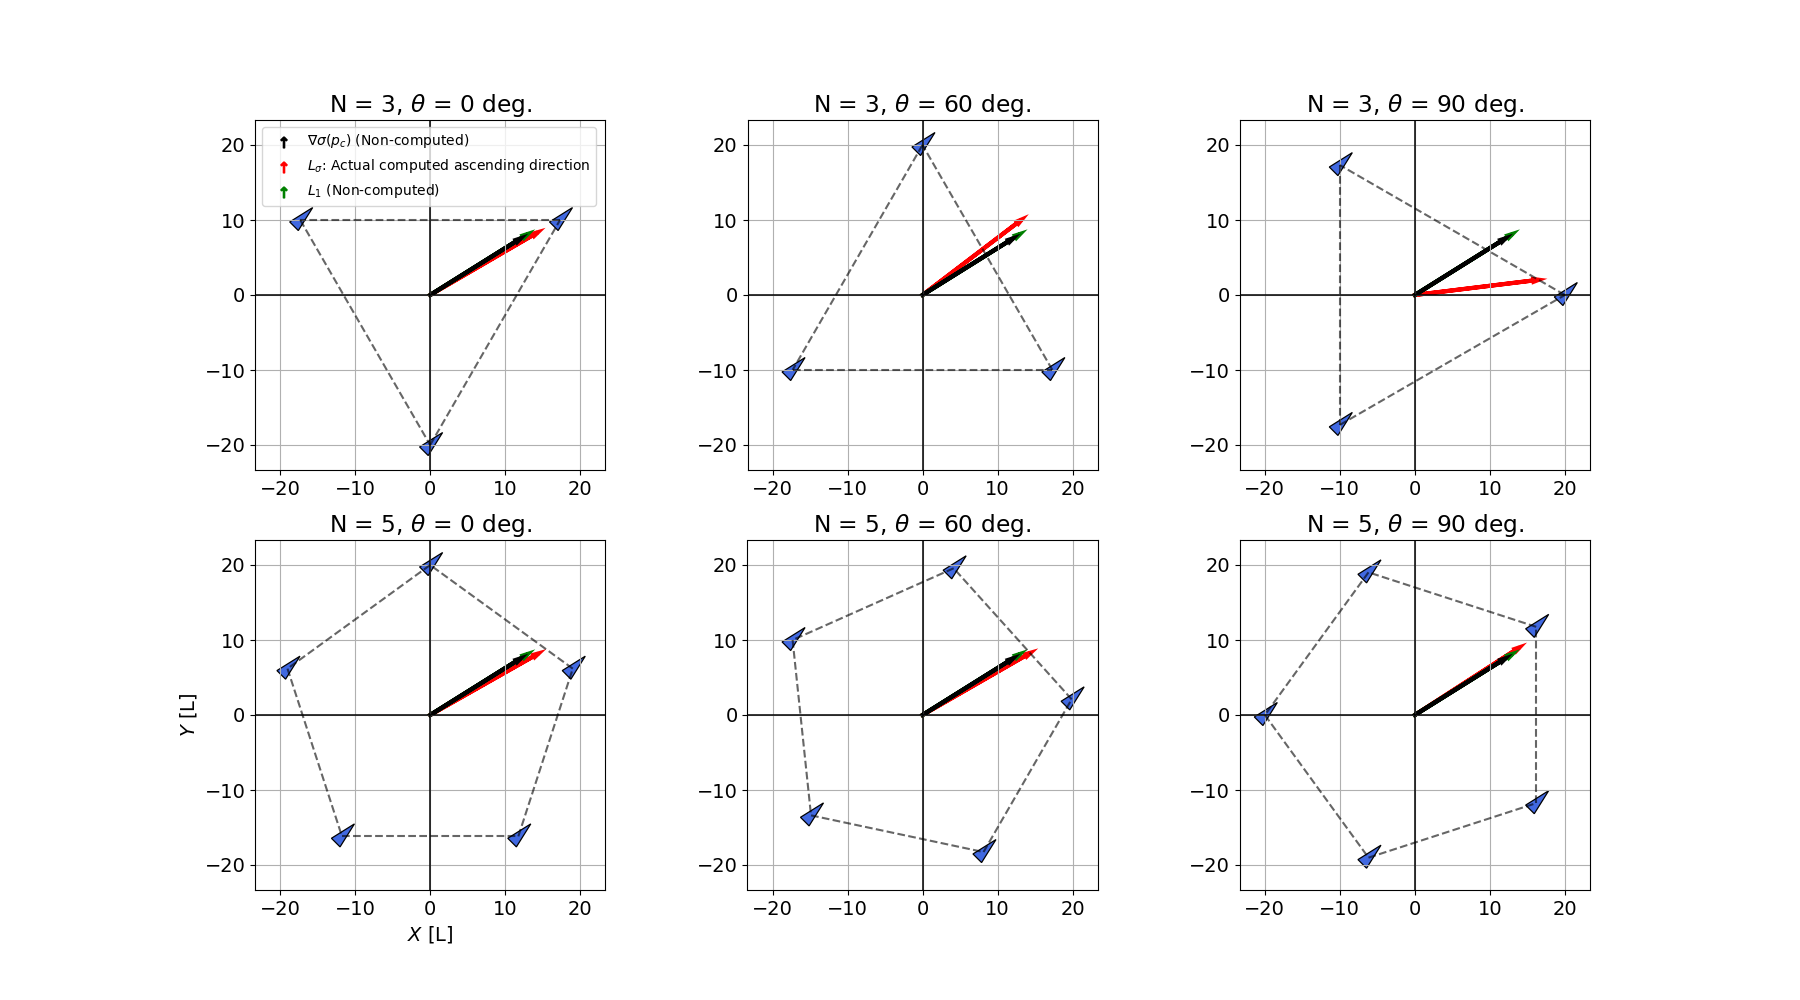
\includegraphics[trim={0 0 0 0}, clip, width=1\columnwidth]{./fig/prop3.png}
\caption{Dadas dos formaciones $x = x^{N\text{poly}}$ sometidas a distintas rotaciones con respecto a $p_c$, en esta figura se muestra el cómputo de $L^1_\sigma(p_c, x^{N\text{poly}})$ y $L_\sigma(p_c, x^{N\text{poly}})$. Véase que, para ambas formaciones, $L^1_\sigma(p_c, x^{N\text{poly}})$ es paralelo al gradiente y completamente invariante.}
\label{fig: ss_prop3}
\end{figure}  

\newpage

Esta proposición es trivial si nos fijamos en que el ángulo $\theta$ que aparece en (\ref{eq: L1theta}) es completamente arbitrario, pues depende del sistema de referencia seleccionado. No obstante, es importante haberla formalizardo para poder seguir adelante con nuestro razonamiento lógico.

Con este resultado en mente, ahora solo necesitamos enfocarnos en los efectos de $U$ y $\Sigma$ de la transformación afín sobre la distribución $x^{N\text{poly}}$.

\vspace{0.2cm}

\begin{prop} \label{pro: usu}
Consideremos la descomposición SVD $A = U\Sigma V^T$, entonces

\begin{equation}
L^1_\sigma(p_c,(I_N \otimes A) x^{N\text{poly}}) \propto U\Sigma^2U^Tr, \nonumber
\end{equation}

donde $r\in\mathbb{R}^m$ es el vector unitario que marca la dirección del gradiente $\nabla\sigma(p_c)$.
\end{prop}
\begin{proof}
Dado el siguiente cambio de coordenadas $\tilde r = \Sigma U^Tr$ y sabiendo que $L^1_\sigma(p_c, x^{N\text{poly}})$ es invariante bajo rotaciones $(I_N\otimes V^T)x$, nos enfocaremos en aplicar la transformación $(I_N \otimes U\Sigma) x$:

\begin{align}
L^1_\sigma(p_c,(I_N \otimes (U\Sigma)) x^{N\text{poly}}) &\propto \sum_{i=1}^N \Big(r^T U\Sigma x_i\Big)U\Sigma x_i \nonumber \\
&\propto U\Sigma\sum_{i=1}^N \Big(\tilde r^T x_i\Big) x_i \propto U\Sigma \tilde r \nonumber = U\Sigma^2U^Tr,
\end{align}

donde hemos aplicado nuevamente el Lema \ref{le: 4}.
\end{proof}

\begin{rem} \label{rem: usu}
Véase que $P = U\Sigma^2U^T$ es la descomposición unitaria de una matriz semidefinida positiva (algo que no nos sorprendente debido al Lema \ref{le: l1}) que, para formaciones $x^{N\text{poly}}$, depende únicamente de $A$. No obstante, hay que tener en cuenta que para un $x$ genérico, $P$ también dependerá de la matriz de rotación (desconocida a priori) entre $r$ y los ejes donde se define $A$.

\end{rem}

La Proposición \ref{pro: usu} tiene una interesante aplicación práctica. Dado que el $L^1_\sigma$ para formaciones $x^{N\text{poly}}$ sigue la dirección del gradiente, podemos decir que el enjambre dispone de un rango simétrico ($\pm \frac{\pi}{2}$ radianes en 2D) para maniobrar mientras se acerca a la fuente. En particular, según la Proposición \ref{pro: usu}, la formación solo necesita estirar su distribución en la dirección en la que desea maniobrar, es decir, elegir una matriz diagonal $\Sigma$ genérica y establecer $U = I_m$. De este modo, la dirección resultante seguirá el estiramiento ${^\xi\Sigma^2}\;{^\xi\nabla\sigma(p_c)}$, donde $\xi$ denota la representación en los ejes perpendiculares elegidos. 

También conviene recodar que esta propiedad no es cierta para una distribución genérica, pues no se cumplen las condiciones para poder aplicar el Lemma \ref{le: 4}, ni las Propociones \ref{pro: RL1} y \ref{pro: usu}. En 2D, podría ocurrir que un estiramiento genérico de $x$ sea precedido por una matriz de rotación que impida independizar el escalado de las componentes de $L^1_\sigma$ en dos ejes perpendiculares.

\newpage

\begin{figure}[!h]
\centering
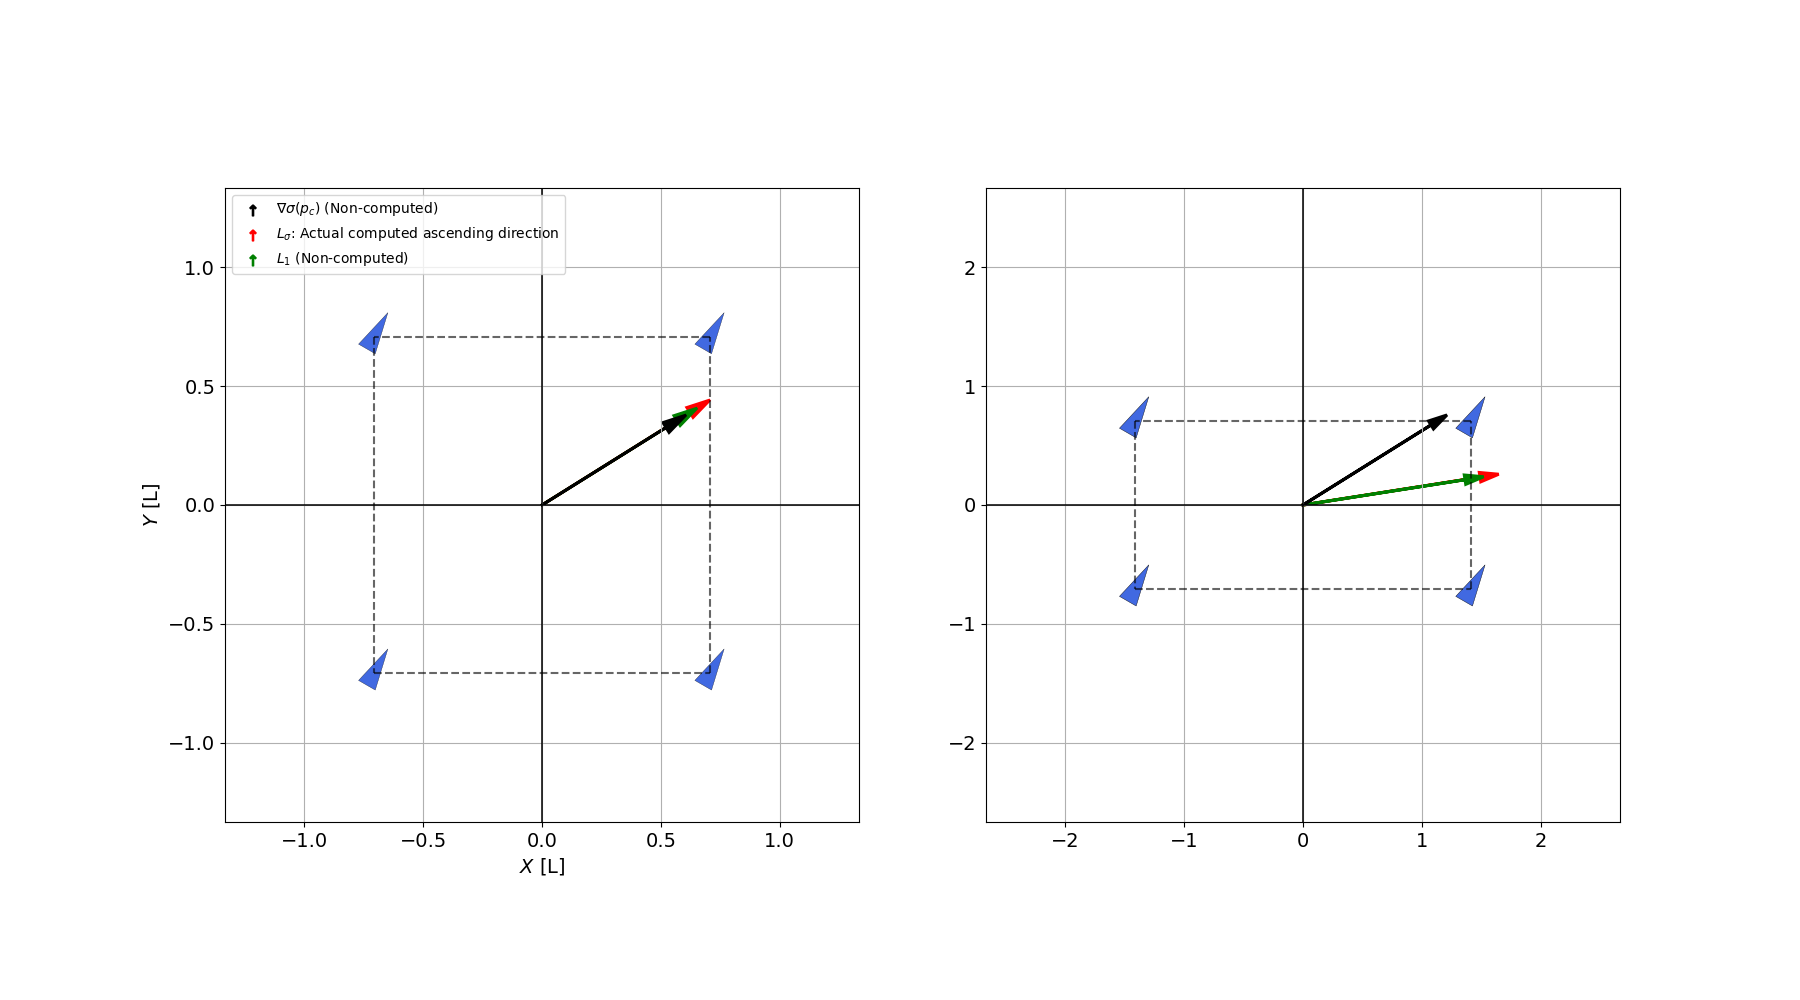
\includegraphics[trim={0 0 0 0}, clip, width=0.85
\columnwidth]{./fig/prop4.png}
\caption{En esta figura, se muestra el cómputo de $L^1_\sigma(p_c, x)$ y $L_\sigma(p_c, x)$ para dos formaciones distintas. Una es $x^{4\text{poly}}$ y la otra es una formación rectangular que puede ser obtenida aplicando una transformación afín de escalado sobre $x^{4\text{poly}}$. Véase que, cuando $x^{4\text{poly}}$ es ensanchada con respecto a un único eje, las proyecciones de $L^1_\sigma(p_c, x)$ y $L_\sigma(p_c, x)$ sobre ese mismo eje también crecen proporcionalmente.}
\label{fig: ss_prop4}
\end{figure} 

A continuación, nos preguntamos cuál sería $L^1_\sigma$ si desplegamos un enjambre compuesto por una gran cantidad de agentes, encerrado dentro de cierto área/volumen y con $x$ siguiendo una distribución genérica $\rho$. Con este análisis, podremos dejar de enfocarnos únicamente en polígonos/poliedros regulares, y comenzar a explorar \textbf{formaciones genéricas} con ciertas simetrías que, como ya veremos más adelante, nos permitirán enunciar una serie de condiciones suficientes para garantizar que $L^1_\sigma$ sea paralelo al gradiente $\nabla\sigma$. 

Cuando $N\to\infty$, nos acercamos al continuo, donde la suma discreta en (\ref{eq: L1.1}) se puede interpretar como una integral si tenemos en cuenta la aproximación de una integral definida con sumas de Riemann. En estos casos, dado que los robots se interpretan como puntos diferenciales, el $N$ de (\ref{eq: L1.1}) se convertirá en el área/volumen encerrado por el perímetro de $x$, es decir, $N = \iiint_{\mathcal{A}} \rho(X,Y,Z) \mathrm{d}X\mathrm{d}Y\mathrm{d}Z$, donde $\mathcal{A}$ es la superficie/volumen correspondiente, y $\rho: \mathbb{R}^m \to \mathbb{R}^+$ es la función de densidad de probabilidad \cite{mendenhall2012introduction} de los robots. Dicha función $\rho$ puede ser, por ejemplo, igual en todas partes para distribuciones uniformes, o similar a una serie geométrica como se ilustra en la Proposición \ref{prop: cross}. Conviene resaltar que las coordenadas $x$ tendrán su origen en la media de $\rho(X,Y,Z)$ en $\mathcal{A}$.

%----

Para ser más concisos, nos centraremos únicamente en el caso 2D, y para mayor claridad en la notación, denotaremos $x_i^X$ y $x_i^Y$ simplemente como $X$ e $Y$. En consecuencia, para el caso de un enjambre de robots siguiendo una función de densidad de probabilidad $\rho(X,Y)$ dentro de una forma/superficie genérica $\mathcal{A}$, la dirección de ascenso $L_\sigma^1(p_c, x)$ se puede calcular como

\begin{align} 
    L_\sigma^1(p_c, x)  & = 
    \frac{||\nabla\sigma(p_c)||}{A}  \iint_\mathcal{A} \rho(X,Y) \left(
    \begin{bmatrix}\cos(\theta) & \sin(\theta) \end{bmatrix} 
    \begin{bmatrix}x_i^X \\ x_i^Y \end{bmatrix}
    \right)
    \begin{bmatrix}x_i^X \\ x_i^Y \end{bmatrix} 
    \mathrm{d}X \mathrm{d}Y
    \nonumber \\
    & = \frac{||\nabla\sigma(p_c)||}{A} \iint_\mathcal{A}  \rho(X,Y)  \begin{bmatrix}
        X^2 \cos(\theta) + XY\, \sin(\theta) \\
        Y^2 \sin(\theta) + XY\, \cos(\theta) \\
    \end{bmatrix}
    \mathrm{d}X \mathrm{d}Y, \nonumber
\end{align}

donde, en lugar de $D$, tenemos $A = \iint_{\mathcal{A}} \rho(X,Y) \mathrm{d}X\mathrm{d}Y$, que es el área de $\mathcal{A}$ en unidades [\emph{longitud $\times$ longitud}]. De modo que será suficiente tener las integrales $\iint_\mathcal{A} \rho(X,Y)XY \mathrm{d}X\mathrm{d}Y$ y $\iint_\mathcal{A} \rho(X,Y)(X^2 - Y^2) \mathrm{d}X\mathrm{d}Y$ iguales a cero para que $L^1_\sigma(p_c,x)$ sea paralelo al gradiente $\nabla\sigma(p_c)$. Teniendo esto en mente, se puede llegar al siguiente resultado.

\vspace{0.2cm}

\begin{prop} \label{pro: U}
Sea una señal $\sigma$, un enjambre con una formación $x$ que consta de $N\to\infty$ robots siguiendo una función de densidad de probabilidad $\rho(X,Y)$ dentro de una superficie $\mathcal{A}$, y un sistema de coordenadas cartesianas $(X-Y)$ arbitrario con origen en el centroide de la formación $p_c$. Diremos que la dirección de ascenso $L_\sigma^1(p_c, x)$ es paralela al gradiente $\nabla\sigma(p_c)$ si la función de densidad de probabilidad $\rho(X,Y)$ para las posiciones de los robots y la superficie $\mathcal{A}$ cumplen las siguientes simetrías:
\begin{enumerate}
\item[S0)] La función de densidad de probabilidad $\rho(X,Y)$ tiene simetría de reflexión (función par) con respecto a al menos uno de los ejes $(X-Y)$, por ejemplo, $\rho(X,Y) = \rho(-X,Y)$.
\item[S1)] La superficie $\mathcal{A}$ tiene simetría de reflexión respecto al mismo eje que en S0.
\item[S2)] Para cada cuadrante de $(X-Y)$, la función de densidad $\rho(X,Y)$ tiene simetría de reflexión con respecto a la bisectriz del cuadrante.
\item[S3)] La superficie $\mathcal{A}$ tiene simetría de reflexión respecto al los mismos ejes que en S2.
\end{enumerate}
\end{prop}

\begin{proof}
En primer lugar, abordamos el caso de $h_1(X,Y) = XY$ y posteriormente el de $h_2(X,Y) = X^2 - Y^2$. Sin pérdida de generalidad, asumimos que la simetría de reflexión es en el eje $Y$; por lo tanto, tenemos que $h_1(X,Y) = -h_1(-X,Y)$ y $\rho(X,Y) = \rho(-X,Y)$. Gracias a esta simetría, también es factible asumir que los límites de integración de $\mathcal{A}$ son simétricos para el eje $X$, tal y como se muestra en la \autoref{fig: obs_xxyy}(a). De este modo, tenemos que

\begin{align*}
\iint_{\mathcal{A}} \rho(X,Y) XY \; \mathrm{d}X \mathrm{d}Y 
&= 
\int_{-t_\beta}^{t_\beta}\int_{0}^{\beta(X)} \rho(X,Y) XY \, \mathrm{d}X  \mathrm{d}Y
+
\int_{-t_\alpha}^{t_\alpha}\int_{\alpha(X)}^{0} \rho(X,Y) XY \, \mathrm{d}X \mathrm{d}Y
\\ & = 
\int_{-t_\beta}^{t_\beta} X F(X,\beta(X)) \, \mathrm{d}X
-
\int_{-t_\alpha}^{t_\alpha} X F(X,\alpha(X)) \, \mathrm{d}X = 0,
\end{align*}

siempre y cuando $\alpha(X)$ y $\beta(X)$ sean funciones pares. Expliquemos este paso con más detalle; en primer lugar, hay que tener en cuenta que

\begin{align*}
F(X,Y) = \int \rho(X,Y) Y \; \mathrm{d}Y 
\end{align*}

siempre va a cumplir que $F(X,Y) = F(-X,Y)$, pues $\rho(X,Y) = \rho(-X,Y)$. Lo que no se tiene por qué cumplir es $F(X,Y) = F(X,-Y)$; no obstante, teniendo en cuenta que la composición de una función par con otra impar es siempre par, dado $g(X) = F(X,f(X))$, si $f(X)$ es par entonces $g(X) = g(-X) \; \Longrightarrow \; F(X,f(X)) = F(-X,f(-X))$. Es decir, aplicado a nuestro caso particular, si $\alpha(X)$ y $\beta(X)$ son pares entonces $F(X,\alpha(X))$ y $F(X,\beta(X))$ también van a ser pares. Finalmente, teniendo en cuenta que el producto de una función por otra impar da como resultado una función impar, y que la integral de una función impar en un rango de integración simétrico siempre es nula. Es directo llegar a la conclusión de que $\iint_\mathcal{A} \rho(X,Y)XY \mathrm{d}X\mathrm{d}Y = 0$

\newpage

\begin{figure}[!h]
\centering
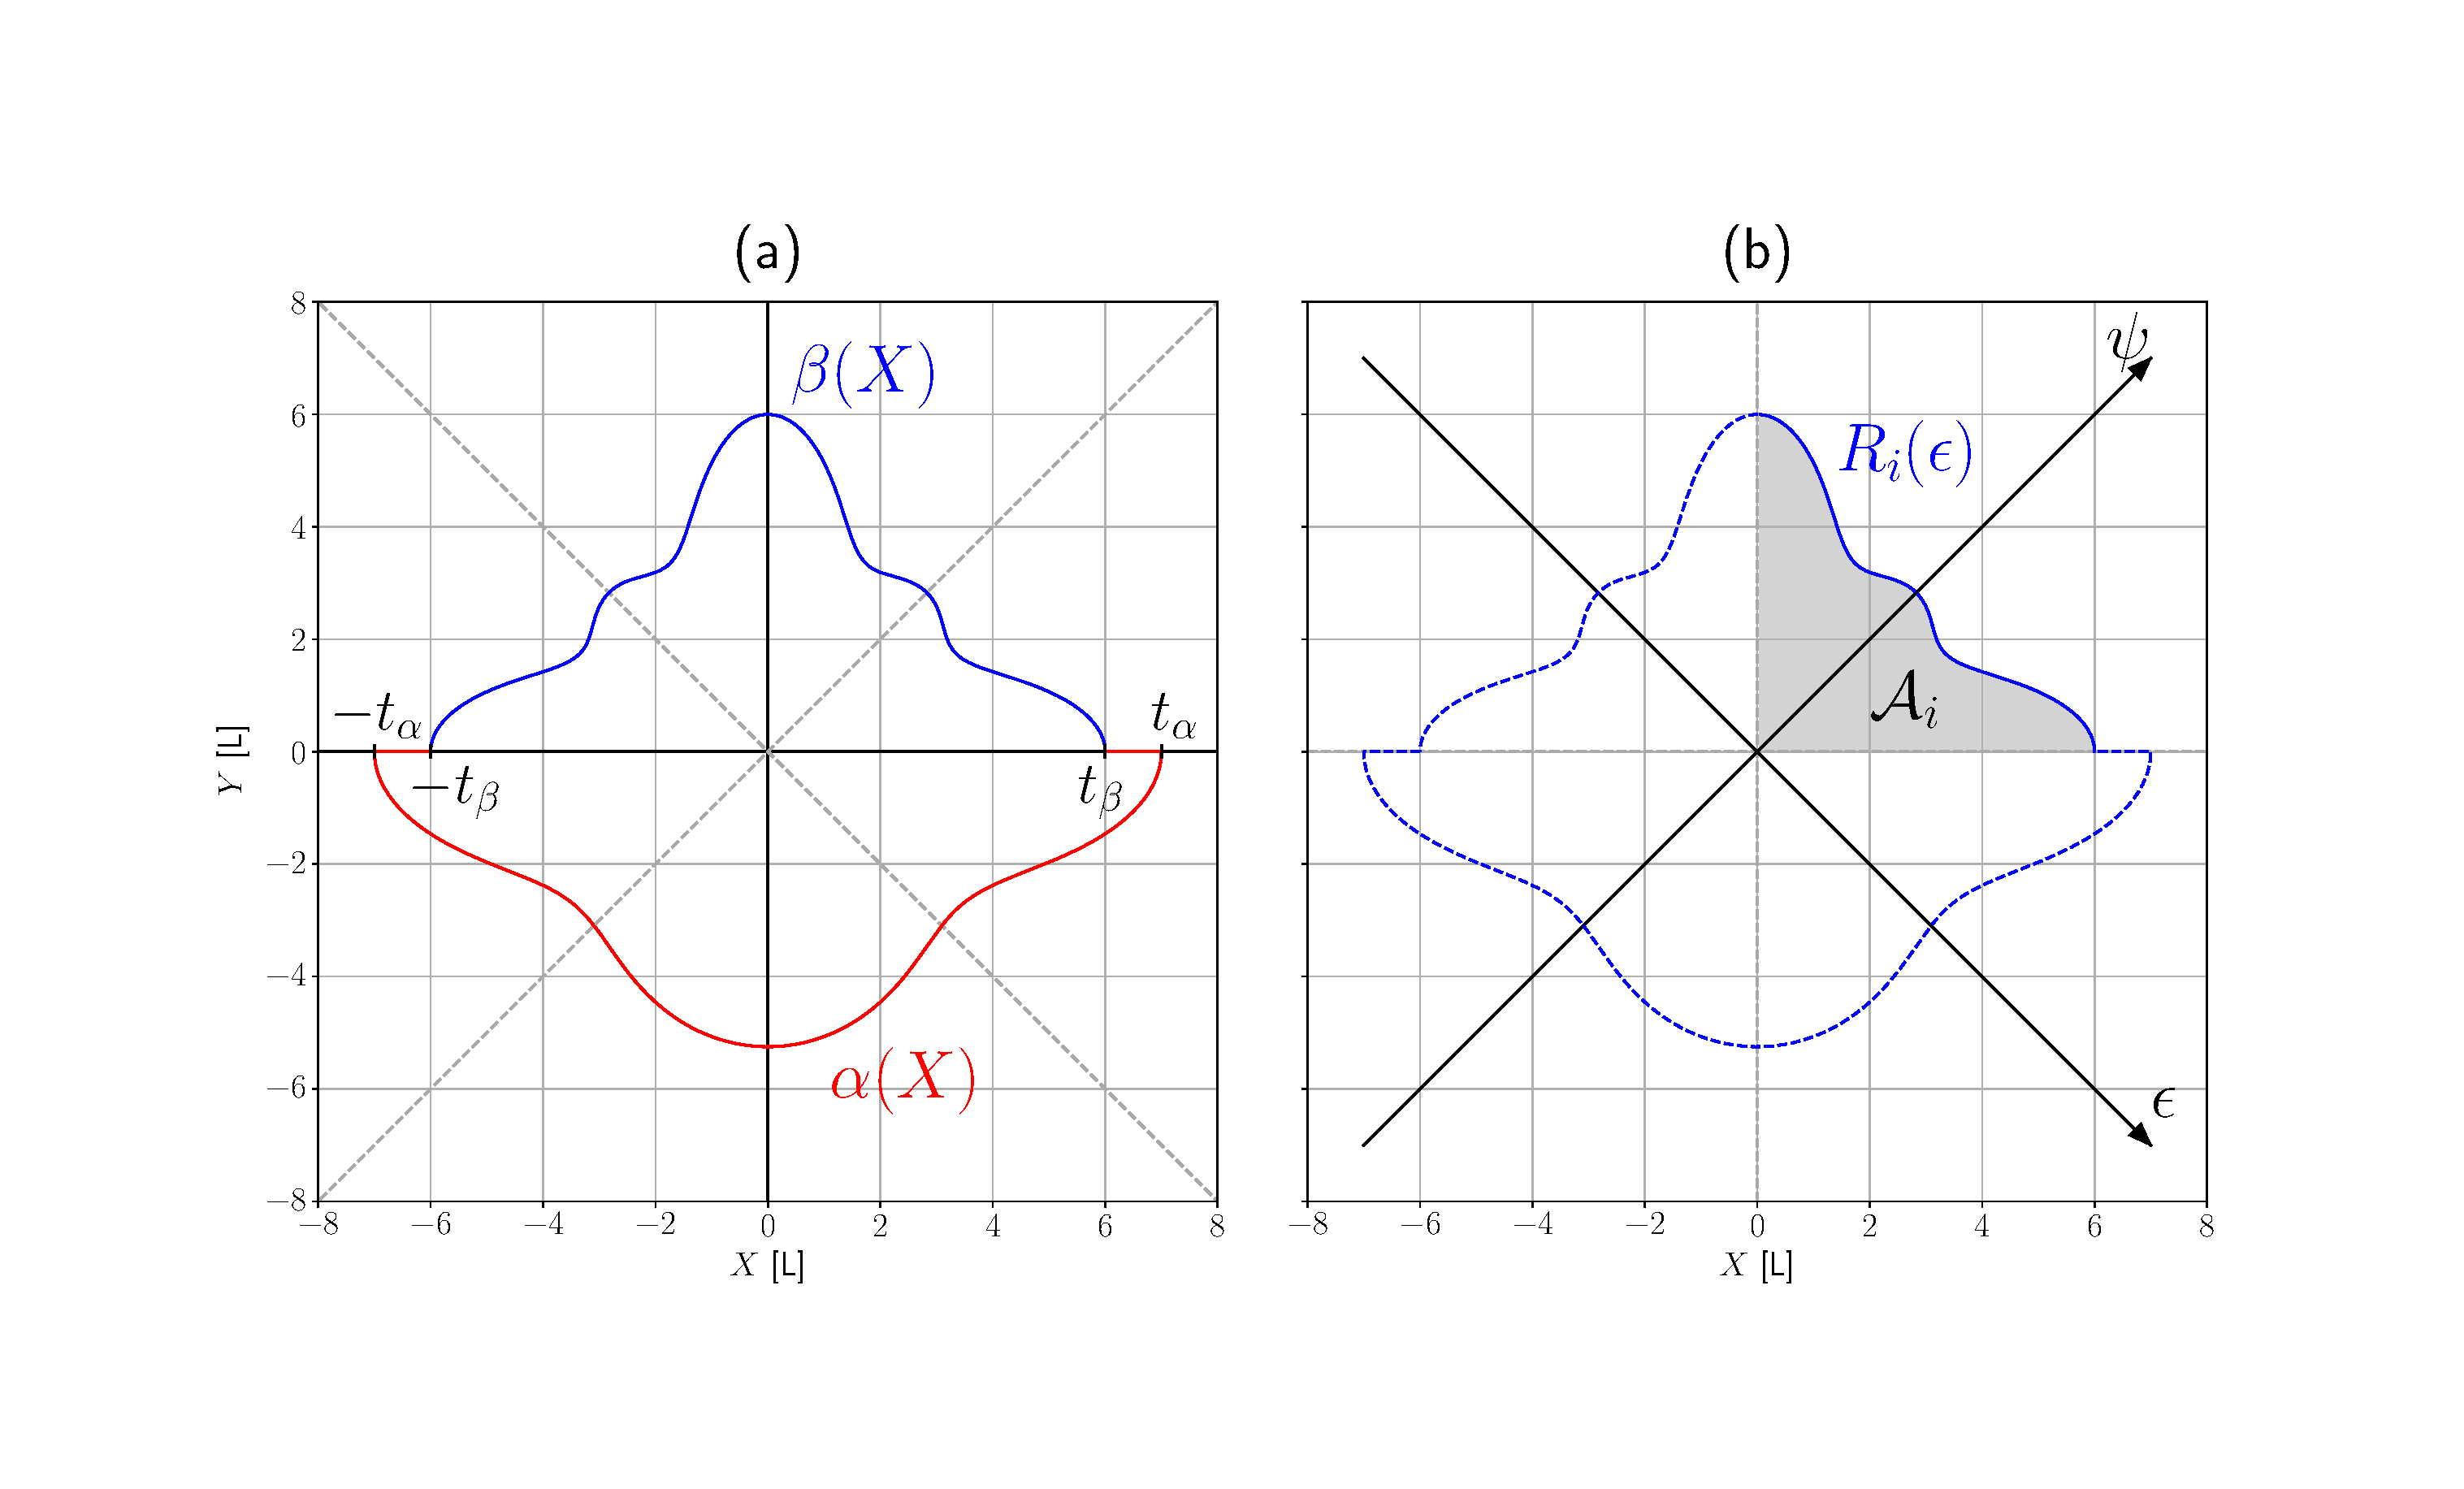
\includegraphics[trim={1cm 3.0cm 1.0cm 4.0cm}, clip, width=1\columnwidth]{./fig/obs_xxyy.eps}
\caption{Ilustración de las dos simetrías referentes al área $\mathcal{A}$, S1 a la izquierda y S3 a la derecha. Dicha $\mathcal{A}$ hace referencia a la superficie que encierra a un enjambre compuesto por $N\to\infty$ robots, distribuidos siguiendo una función de densidad de probabilidad $\rho(X,Y)$ que debería respetar S0 y S2.}
\label{fig: obs_xxyy}
\end{figure}

A continuación, analizaremos la integral de $h_2(X,Y)$, sumando a todas las simetrías anteriores S2 y S3. En primer lugar, hay que tener en cuenta que 

\begin{align*}
\iint_{\mathcal{A}} \rho(X,Y) h_2(X,Y) \; \mathrm{d}X \mathrm{d}Y 
=
\sum_{i=1}^4
\iint_{\mathcal{A}_i} \rho(X,Y) h_2(X,Y) \; \mathrm{d}X \mathrm{d}Y,
\end{align*}

donde $\mathcal{A}_i$ denota el área del cuadrante $i \in \{1,2,3,4\}$. Es decir, si conseguimos demostrar que la integral de $h_2(X,Y)$ sobre $\mathcal{A}_i$ es nula para todos los cuadrantes, entonces la integral de $h_2(X,Y)$ sobre $\mathcal{A}$ también lo será. Con esto en mente, aplicaremos el cambio de variable $g(\epsilon,\psi) = (\psi + \epsilon, \psi - \epsilon)/\sqrt{2}$, que corresponde a una rotación de $+\pi/2$ radianes del plano $(X-Y)$. De este modo, sabiendo que $\int_{A} f(x,y) = \int_{B} (f \circ g) |J_g|$, donde $|J_g| = |\begin{bmatrix}\nabla g_1 & \nabla g_2 \end{bmatrix}^T| = \sqrt{2}$, y que gracias a S2 y S3 tenemos límites de integración simétricos en $\epsilon$ y $\rho(\epsilon,\psi) = \rho(-\epsilon,\psi)$, entonces

\begin{align*}
\iint_{\mathcal{A}_i} \rho(X,Y) h_2(X,Y) \; \mathrm{d}X \mathrm{d}Y
&= 
2 \sqrt{2} \iint_{\mathcal{B}_i} \rho(\epsilon,\psi) \epsilon \psi \; d\epsilon d\psi
\\ &= 
2 \sqrt{2} \int_{-t_i}^{t_i}\int_{|\epsilon|}^{R_i(\epsilon)} \rho(\epsilon,\psi) \epsilon \psi \; d\epsilon d\psi
\\ &= 
2 \sqrt{2} \int_{-t_i}^{t_i} \epsilon \left [F(\epsilon,R_i(\epsilon)) - F(\epsilon,|\epsilon|) \right ] d\epsilon
= 0,
\end{align*}

\newpage
siempre y cuando $R_i(\epsilon) = R_i(-\epsilon)$; lo que equivale a decir que $\alpha(X)$ tenga reflexión especular con respecto respecto al bisector dentro de los dos cuadrantes superiores, y que $\beta(X)$ cumpla los mismo pero para los dos cuadrantes inferiores. Téngase en cuenta que evidentemente $|\epsilon|$ también es una función par.

\end{proof}

Es interesante tener en cuenta que $\iint_\mathcal{A} \rho(X,Y)XY \mathrm{d}X\mathrm{d}Y$ se puede separar en $\iint_\mathcal{A} \rho(X,Y)X \mathrm{d}X = X_{c}$ y $\iint_\mathcal{A} \rho(X,Y)Y \mathrm{d}Y = Y_{c}$, donde $X_c$ e $Y_c$ son las coordenadas del centroide de la distribución en el plano $(X-Y)$; y que $\iint_\mathcal{A} \rho(X,Y)(X^2 - Y^2) \mathrm{d}X\mathrm{d}Y = \text{VAR}_\mathcal{A}[X] - \text{VAR}_\mathcal{A}[Y]$, donde $\text{VAR}_\mathcal{A}[X]$ es la varianza de la distribución con respecto a un eje arbitrario $X$. Es decir, cuando la integral en $h_1(X,Y)$ sea nula, significará que la coordenada del centroide en el eje perpendicular al eje de simetría es nula; mientras que si la integral en $h_2(X,Y)$ es nula, tendremos que $\text{VAR}_\mathcal{A}[X] = \text{VAR}_\mathcal{A}[Y]$.

La Proposión \ref{pro: U} es un resultado muy potente, pues nos permite asegurar que la dirección de ascenso $L_\sigma^1(p_c, x)$ es siempre paralela al gradiente $\nabla\sigma(p_c)$ para una familia de formaciones mucho más amplia que $x^{N\text{poly}}$ (ver \autoref{fig: prop5}). Es más, resulta interesante observar que si tomamos el área que encierra cualquier formación $x^{N\text{poly}}$ y suponemos, por ejemplo, una distribución uniforme (ver $x^{\text{rct}}$ en la \autoref{fig: 4rect}), entonces la Proposición \ref{pro: U} nos dice lo mismo que el Lema \ref{le: 4}. Este echo nos motiva a pensar que, en cierto modo, siempre que una formación discreta cumpla unas simetrías similares a las de la Proposición \ref{pro: U}, tendremos que la dirección de $L_\sigma^1(p_c, x)$ es muy próxima a la del gradiente $\nabla\sigma(p_c)$.

\begin{figure}[!h]
\centering
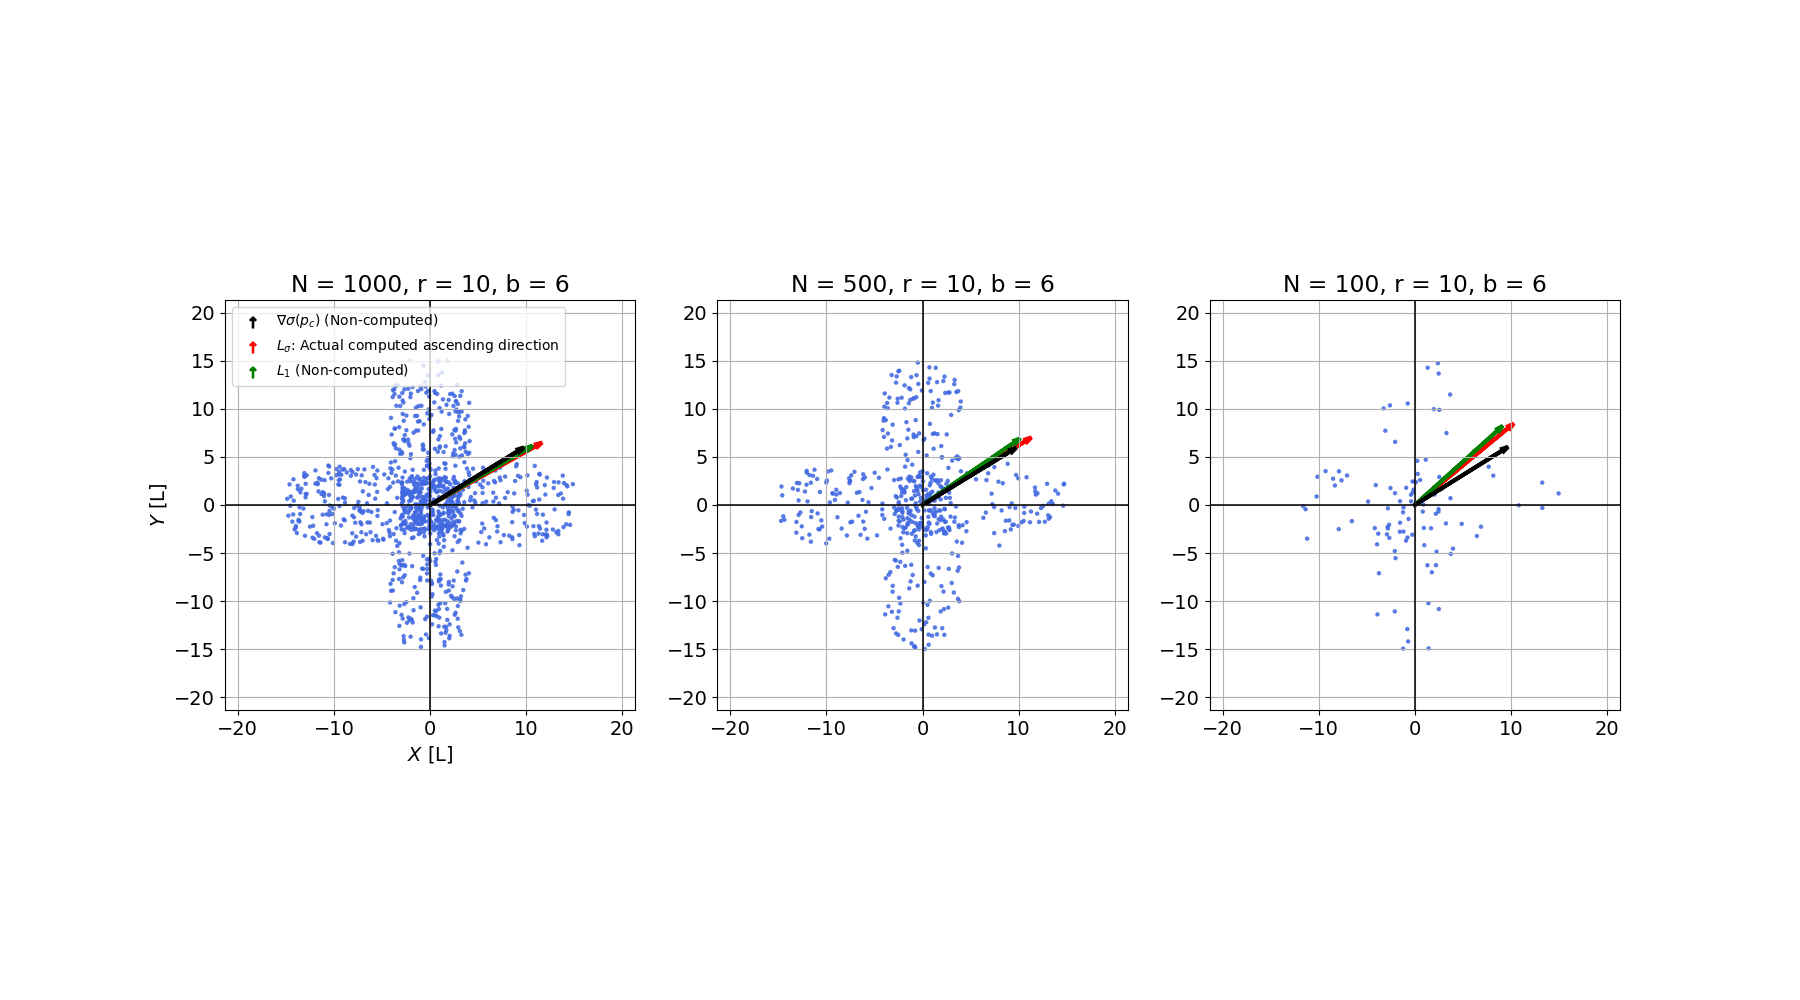
\includegraphics[trim={3cm 5.0cm 3cm 5.0cm}, clip, width=1\columnwidth]{./fig/prop5.png}
\caption{En esta figura tenemos tres formaciones, con grandes diferencias en cuanto a número de agentes $N$, pero encerradas en un mismo perímetro $\mathcal{A}$ y siguiendo una misma función de densidad $\rho(X,Y)$. Dado que se cumplen todas las simetrías de la Proposición \ref{pro: U}, podemos visualizar que según $N$ aumenta, es decir $N$ comienza a tender a $\infty$, $L_\sigma^1(p_c, x)$ es cada vez más paralelo al gradiente $\nabla\sigma(p_c)$.}
\label{fig: prop5}
\end{figure}

Para finalizar esta subsección, conviene analizar lo que sucede cuando únicamente se cumplen las simetrías S0 y S1, es decir $\text{VAR}_{\mathcal{A}}[X] \neq \text{VAR}_{\mathcal{A}}[Y]$. En estos casos, tendremos que

\begin{align*} 
    L_\sigma^1(p_c, x)  = 
     \frac{||\nabla\sigma(p_c)||}{A} \begin{bmatrix}
        \text{VAR}_{\mathcal{A}}[X] \cos(\theta)\\
        \text{VAR}_{\mathcal{A}}[Y] \sin(\theta)\\
    \end{bmatrix},
\end{align*}

de modo la varianza en un eje modulará la proyección de $L_\sigma^1(p_c, x)$ sobre ese mismo eje. Suponiendo una formación de este estilo, como la que se muestra en la \autoref{fig: batman}, podemos comprobar que esta característica es muy interesante, pues escalando la formación en direcciones paralelas o perpendiculares al eje de simetría podemos maniobrar al enjambre mientras se garantiza que $L_\sigma^1$ sigue siendo una dirección de ascenso. Esta es una herramienta que, por ejemplo, permitirá al enjambre evitar obstáculos y adaptarse a escenarios desconocidos mientras $p_c$ sigue tendiendo a la fuente de $\sigma$. 

\vspace{0.8cm}

\begin{figure}[!h]
\centering
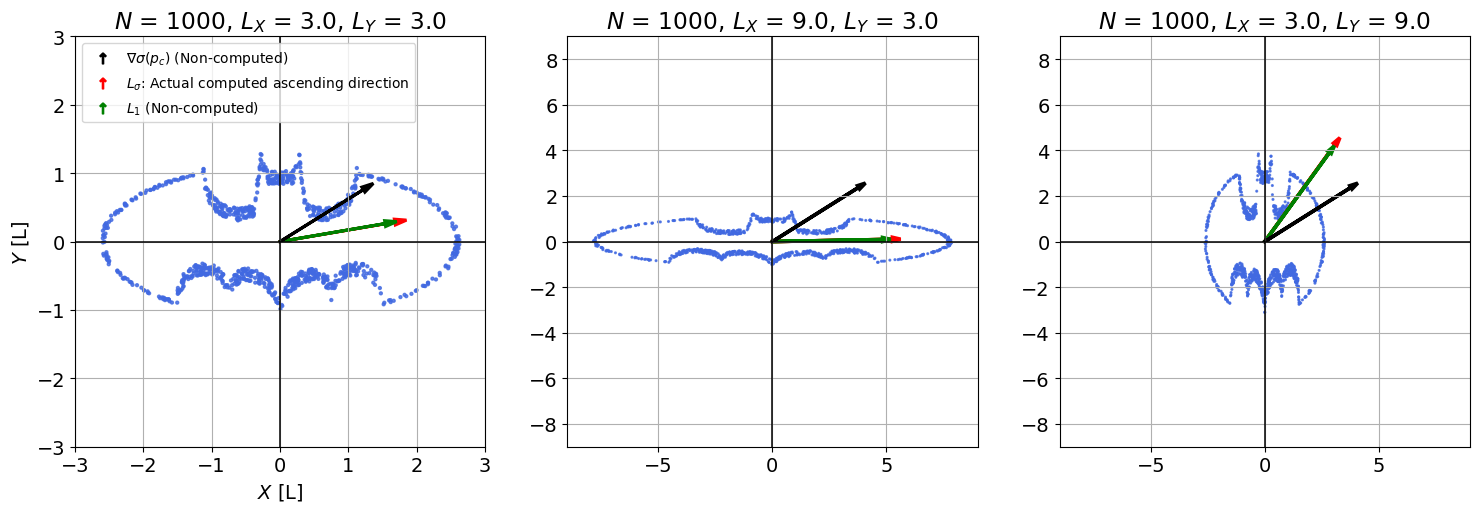
\includegraphics[trim={0cm 0.0cm 0cm 0.0cm}, clip, width=1\columnwidth]{./fig/batman.png}
\caption{Tenemos a un enjambre con un número fijo de agentes $N$ que trata de de dibujar el logo de Batman, generando una formación con simetría especular respecto a $Y$. En esta figura, se computa $L_\sigma^1$ y $L_\sigma$ para observar cómo varían dichos vectores ante distintos escalados de la formación en los ejes $X$ e $Y$. Notamos que cuando la varianza aumenta en un eje, la componente paralela a dicho eje de $L_\sigma^1$ también lo hace de forma proporcional y, por supuesto, $L_\sigma$ le acompaña.}
\label{fig: batman}
\end{figure}

\vspace{0.2cm}

% Estimación distribuida del centroide
%%%%%%%%%%%%%%%%%%%%%%%%%%%%%%%%%%%%%%%%%%%%%%%%%%%%%%%%%%%

\subsubsection{Estimación distribuida del centroide}

Terminamos la sección de herramientas de \textit{source-seeking} con un algoritmo que permitirá a los robots estimar el centroide de la formación. El objetivo final es presentar un resultado que permita calcular todo $x_i$, es decir, la posición del centroide $p_c$ desde el sistema de referencia propio de cada robot.

El algoritmo que nosotros propondremos surge de una colección de resultados bien establecidos en el control de formación, pues este tipo de técnicas tienen su dual en el problema de localización relativa \cite{oh2015survey}. En particular, suponiendo que algunos robots del enjambre (más adelante detallaremos a qué nos referimos con ''algunos'') puedan medir sus distancias relativas, entonces podemos considerar la siguiente ley de localización:

\begin{equation} \label{eq: esti}
\frac{\mathrm{d}}{\mathrm{dt}} {\hat x_i}(t) = -\sum_{j\in\mathcal{N}_i} \Big((\hat x_i(t) - {\hat x}_j(t)) - (x_i - x_j) \Big), \; \forall i\in\mathcal{V},
\end{equation}


\newpage

donde $(x_i - x_j)$ es el término fijo de la medición hardware, que es equivalente a la posición relativa $(p_i - p_j)$; y $\hat x_i\in\mathbb{R}^m$ es el término dinámico es el valor software, que corresponderá a la estimación de la posición del centroide desde el robot $i$. Téngase en cuenta que, dado que $\hat x_j$ es un valor de software, entonces necesita ser comunicado al robot $i$ para todo $(i,j)\in\mathcal{E}$. A continuación, propondremos un resultado que estudia todas aquellas soluciones de \eqref{eq: esti} que nos permitirán estimar $x_i$.

\vspace{0.3cm}

\begin{prop}
La estimación $\hat x_i$ en (\ref{eq: esti}) converge de forma exponencialmente rápida al valor actual $x_i$ a medida que $t\to\infty$ si y solo si $\sum_i^N\hat x_i(0) = 0$.
\end{prop}

\begin{proof}
En primer lugar, recordemos que el tipo de grafo $\mathcal{G}$ considerado para los siguientes resultados es no dirigido y conectado. Con esto en mente, escribamos la forma compacta de (\ref{eq: esti}) como

\begin{align} \label{eq: estidelta}
\frac{\mathrm{d}}{\mathrm{dt}} \hat x(t) = - \overline L\hat x(t) + \overline Lx \quad
\Rightarrow \quad \frac{\mathrm{d}}{\mathrm{dt}} \hat x(t) + \overline L\hat x(t) = \delta, 
\end{align}

donde $L$ es la matriz Laplaciana (\ref{eq: L}), y $\delta = \overline Lx = \overline Lp \in \mathbb{R}^{m|\mathcal{E}|}$ es el vector apilado de las posiciones relativas $(x_i-x_j) = (p_i - p_j), (i,j)\in\mathcal{E}$. Notamos que la dinámica de $\sum_i^N\hat x_i(t)$ es estacionaria, es decir, $\sum_i^N \frac{\mathrm{d}}{\mathrm{dt}}\hat x_i(t) = 0$, ya que

\begin{equation}\label{eq: invcen}
\mathbf{1}^T_{mN} \left(-\overline L\hat x(t) + \overline Lx\right) = 0,
\end{equation}

en vista de (\ref{eq: L}) y teniendo en cuenta que $B^T\mathbf{1}_N = 0$. Por lo tanto, si $\sum_i^N\hat x_i(0) = 0$, el centroide de $\hat x(t)$ permanecerá en cero para todo $t$. Tenga en cuenta que esta es una condición suficiente y también necesaria para garantizar la invarianza del centroide de $\hat x(t)$, ya que $\mathbf{1}^T_{N}$ es el autovector de $L$ asociado a su único autovalor nulo. También sabemos que la trayectoria eventual $\hat x^h(t)$ de la parte homogénea de la ecuación diferencial (\ref{eq: estidelta}) está dada por

\begin{equation} \label{eq: xh}
\lim_{t\to\infty}\hat x^h(t) = c_1 \otimes \mathbf{1}_N,
\end{equation}

ya que $\mathbf{1}_N$ es el autovector asociado al único autovalor cero de $L$, $c_1$ depende de la condición inicial $\hat x(0)$, y el resto de los términos de $\hat x^h(t)$ desaparecen rápidamente de forma exponencial, ya que $L$ es semidefinida positiva\footnote{De hecho, sabemos, a partir del resultado estándar de un protocolo de consenso para grafos no dirigido, que $c_1 = \left( \sum_{i=1}^N\hat x(0) \right) / N$ \cite{olfati2004consensus}; no obstante, este resultado no será necesario para nuestro análisis.}.

Ahora, dado $\overline Lx^p = \delta$, verifiquemos que $\hat x^p = x + \left(c_2 \otimes \mathbf{1}_N\right)$ es una potencial familia de soluciones particulares para (\ref{eq: estidelta}), dependientes de $c_2\in\mathbb{R}^m$. Sumando a la solución homogénea este nuevo término $x^p$, nos queda que

\begin{equation}
\lim_{t\to\infty}\hat x(t) = \Big((c_1 + c_2) \otimes \mathbf{1}_N\Big) + x. \nonumber
\end{equation}

Sin embargo, dado que el centroide de $x$ es cero por definición, y el centroide de $\hat x(0)$ es cero e invariante debido a (\ref{eq: invcen}), debe ser cierto que $(c_1 + c_2) = 0$, es decir, $x$ y $\hat x(t)$ comparten el mismo marco de coordenadas; por lo tanto, llegamos a $\lim_{t\to\infty}\hat x(t) = x$ exponencialmente rápido.

\end{proof}

\vspace{0.2cm}

\begin{figure}[!h]
\centering
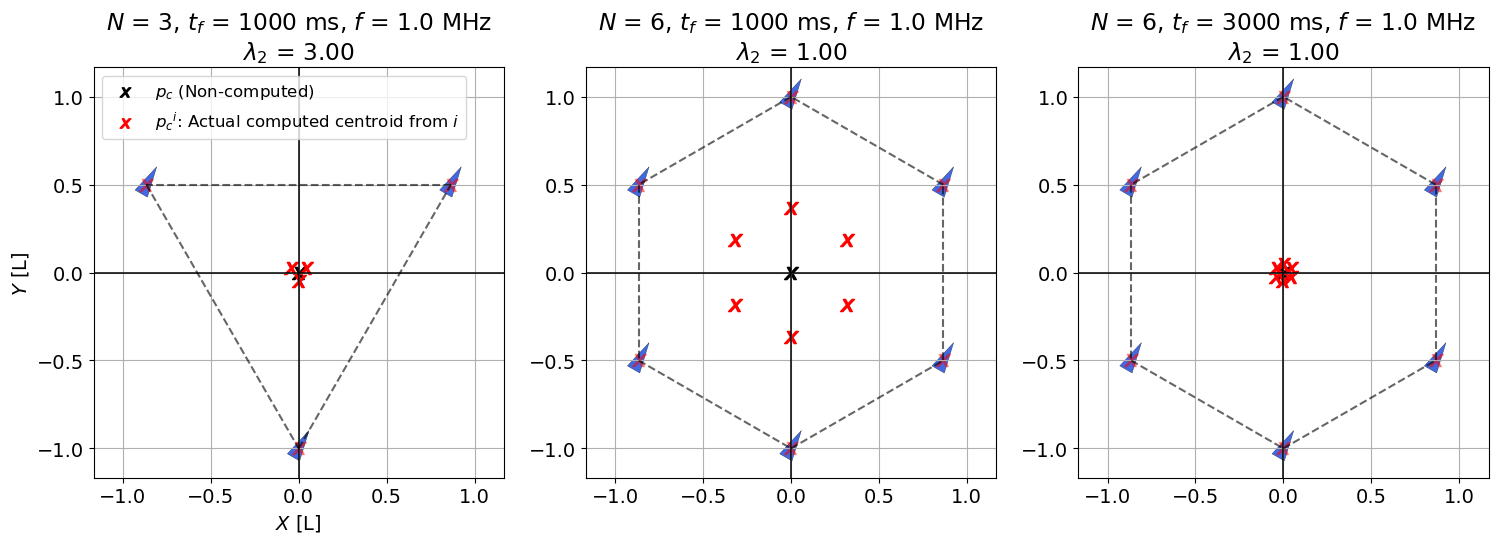
\includegraphics[trim={0cm 0.0cm 0cm 0.0cm}, clip, width=1\columnwidth]{./fig/centroid.png}
\caption{En esta figura se visualiza, para dos formaciones distintas, la estimación del centroide (''x'' roja) realizada por cada uno de los agentes del enjambre. El algoritmo de estimación del centroide se está ejecutando en ambos casos a 1 MHz. Resulta interesante observar que, cuando mayor es la conectividad algebraica del grafo $\lambda_2$, más rápido convergen las estimaciones al valor real del centroide.}
\label{fig: centroid}
\end{figure}

La condición $\sum_{i=1}^N\hat x_i(0) = 0$ se puede satisfacer estableciendo todos los valores iniciales del software $\hat x_i(0) = 0$. Después de que los robots alcancen su formación deseada, si queremos estimar cuándo un grupo calcula su primera dirección ascendente confiable, es importante saber cómo de rápido $\hat x(t)$ tiende a su valor asintótico. Esto está determinado por la conectividad algebraica $\lambda_2$ en $\mathcal{G}$, es decir, el menor autovalor distinto de cero del Laplaciano $L$ \cite{bullo2020lectures}, y por una posible ganancia positiva para (\ref{eq: esti}) (ver \autoref{fig: centroid}). Mientras que $\lambda_2$ está relacionado únicamente con la topología del grafo no dirigido considerado \cite{bullo2020lectures}, la ganancia positiva está relacionada con el ancho de banda disponible y la implementación en tiempo discreto de (\ref{eq: esti}) en hardware; es decir, cuanto más rápido iteremos (\ref{eq: esti}), más rápido será la convergencia $\hat x(t) \to x$.

%%%%%%%%%%%%%%%%
% Simulaciones %
%%%%%%%%%%%%%%%%

\subsection{Simulaciones}

A lo largo de toda la sección anterior, hemos ido mostrado pequeñas simulaciones que han permitido verificar numéricamente cada uno de los resultados expuestos. No obstante, en esta sección dedicada exclusivamente a simulaciones, presentaremos una serie de escenarios mucho más complejos que harán uso de forma simultanea de varias de las herramientas presentadas. Todos los gráficos y simulaciones relacionados con la metodología de \textit{source-seeking} pueden encontrarse en \cite{repo_ss}, un repositorio de GitHub creado y mantenido por el autor de este TFM.

\newpage

\subsubsection*{Sim. I: Un enjambre con una cantidad variable de agentes tratando de encontrar la fuente}

En esta primera misión (\autoref{fig: ss_sim1}), un enjambre de 200 robots con dinámica de integrador simple, distribuidos uniformemente en una formación rectangular, ha de hallar el origen de un campo cuadrático. En su camino hacía la fuente, el equipo se encuentra en t = 15 con un conjunto de 15 nuevos agentes que se unen al enjambre. Sin embargo, en t = 20 algunas baterías empiezan a fallar, lo que produce que un total de 20 agentes se desconecten de la red.

El objetivo de esta misión es demostrar la \textbf{resiliencia} del enjambre ante situaciones en las que, debido a variaciones drásticas el número de agentes, la geometría de la formación se hace muy irregular. A pesar de estas adversidades, el enjambre consigue encontrar la fuente de la señal en t = 41.

\begin{figure}[!h]
\centering
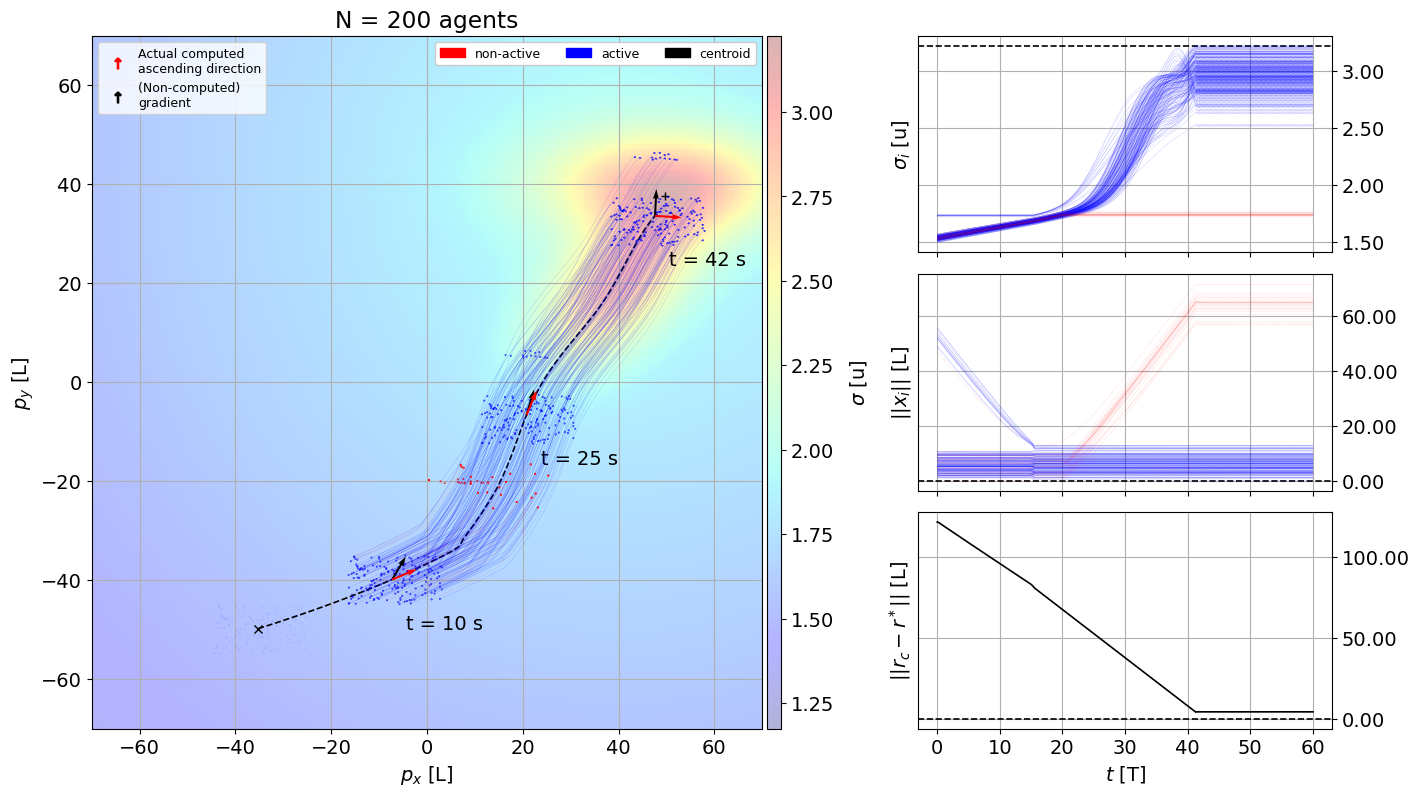
\includegraphics[trim={0cm 0.0cm 0cm 0.0cm}, clip, width=1\columnwidth]{./fig/ss_sim1.png}
\caption{En esta figura tenemos la simulación (I) de un enjambre de robots ejecutando nuestro algoritmo de \textit{source-seeking}. En el gráfico de la izquierda tenemos una representación del escenario virtual que permite visualizar cómo se aproxima el enjambre a la fuente; mientras que en los gráficos de la derecha se visualiza la distancia del centroide a la fuente y, para todo agente $i$, la medición $\sigma_i$ y su distancia al centroide $x_i$.}
\label{fig: ss_sim1}
\end{figure}

\subsubsection*{Sim. II: La geometría del enjambre cambia para esquivar obstáculos}

En esta segunda misión (\autoref{fig: ss_sim2}), otro enjambre de 200 agentes, inicialmente distribuidos de forma uniforme en una circunferencia, debe de encontrar la fuente de una señal gaussiana. A lo largo de su camino, el enjambre se encontrará con una serie de obstáculos, de modo que deberá de aplicar algunos de nuestros resultados para lograr esquivarlos mientras se sigue aproximando a la fuente.

\newpage

El principal objetivo de esta simulación es demostrar el potencial de nuestro algoritmo en términos de \textbf{maniobrabilidad}. Como ya comentados al discutir sobre la Proposición \ref{pro: U}, la varianza de la formación permite modular indirectamente $L_\sigma$, vector que al fin y al cabo se puede traducir como una\textbf{ dirección de guiado} para el enjambre. En este caso concreto, al pasar de una formación circular, donde la varianza es igual en todos los ejes ($L_\sigma^1$ paralelo a $\nabla \sigma$), a una formación rectangular, el enjambre logra aumentar drásticamente la proyección de $L_\sigma$ sobre la horizontal, lo que le permite seguir aproximándose a la fuente mientras esquiva a los obstáculos.

\begin{figure}[!h]
\centering
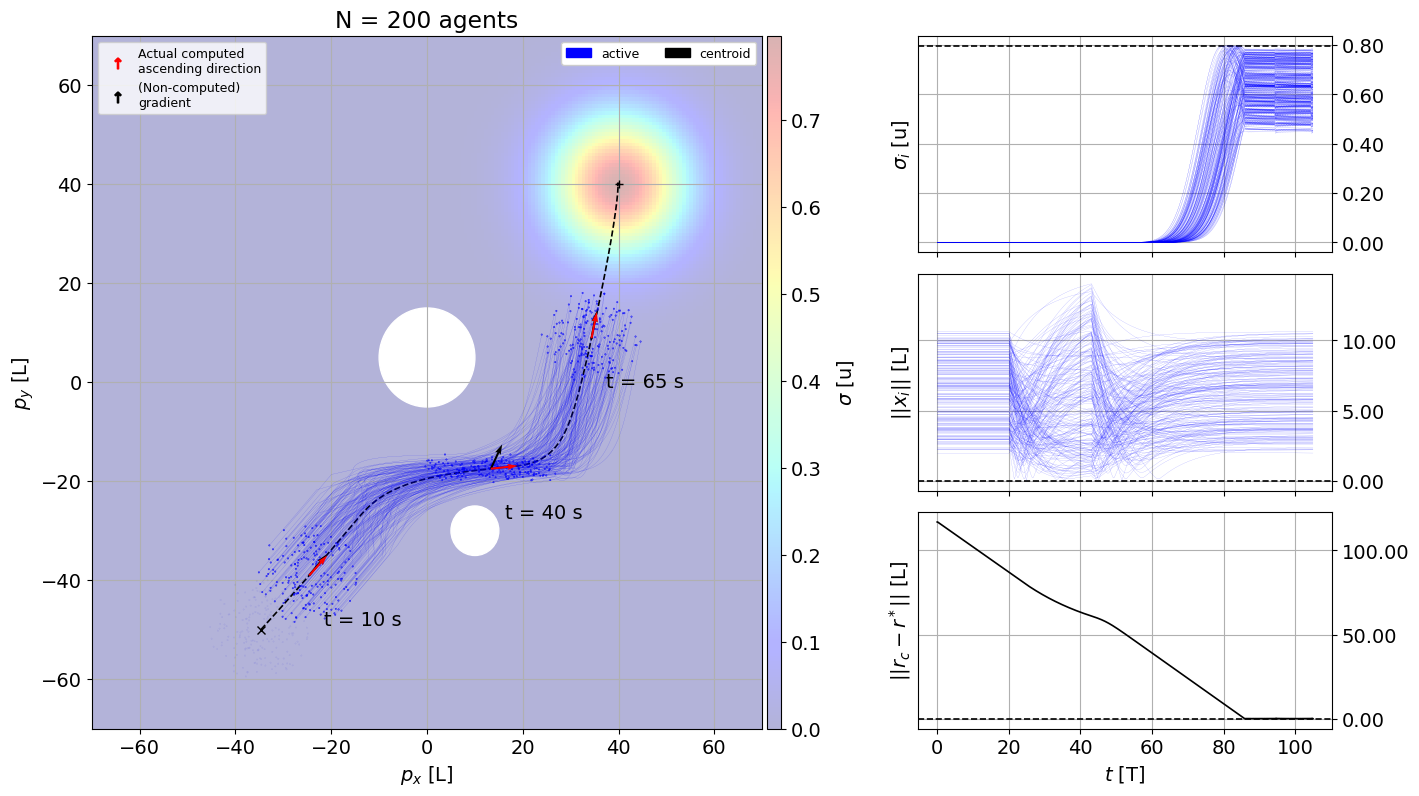
\includegraphics[trim={0cm 0.0cm 0cm 0.0cm}, clip, width=1\columnwidth]{./fig/ss_sim2.png}
\caption{En esta figura tenemos la simulación (II) de un enjambre de robots ejecutando nuestro algoritmo de \textit{source-seeking}. En el gráfico de la izquierda tenemos una representación del escenario virtual que permite visualizar cómo se aproxima el enjambre a la fuente a la vez que esquiva una serie de obstáculos (círculos blancos); mientras que en los gráficos de la derecha se visualiza la distancia del centroide a la fuente y, para todo agente $i$, la medición $\sigma_i$ y su distancia al centroide $x_i$.}
\label{fig: ss_sim2}
\end{figure}

\subsubsection*{Sim. III: El enjambre rota para adaptarse a un terreno desconocido}

En esta tercera misión (\autoref{fig: ss_sim3}), tenemos nuevamente a un enjambre de 200 robots, uniformemente distribuidos en una formación rectangular, que ha de encontrar la fuente de una señal gaussiana. En su camino a la fuente, el enjambre se percata de que debe de rotar drásticamente su dirección de movimiento para, por ejemplo, poder adaptarse al entorno mientras se sigue aproximando a la fuente.

El objetivo de esta simulación vuelve a ser ilustrar las capacidades de nuestro algoritmo en cuanto a maniobrabilidad. En este caso, se parte de una formación con una gran varianza en el eje horizontal, para posteriormente pasar a otra formación que traslada esta varianza superior al eje vertical. Es decir, mediante una rotación de 90º en la formación, el enjambre logra rotar también en la misma magnitud angular $L_\sigma$, que como ya hemos comentado anteriormente, se puede interpretar como un vector de guiado.

\newpage

\begin{figure}[!h]
\centering
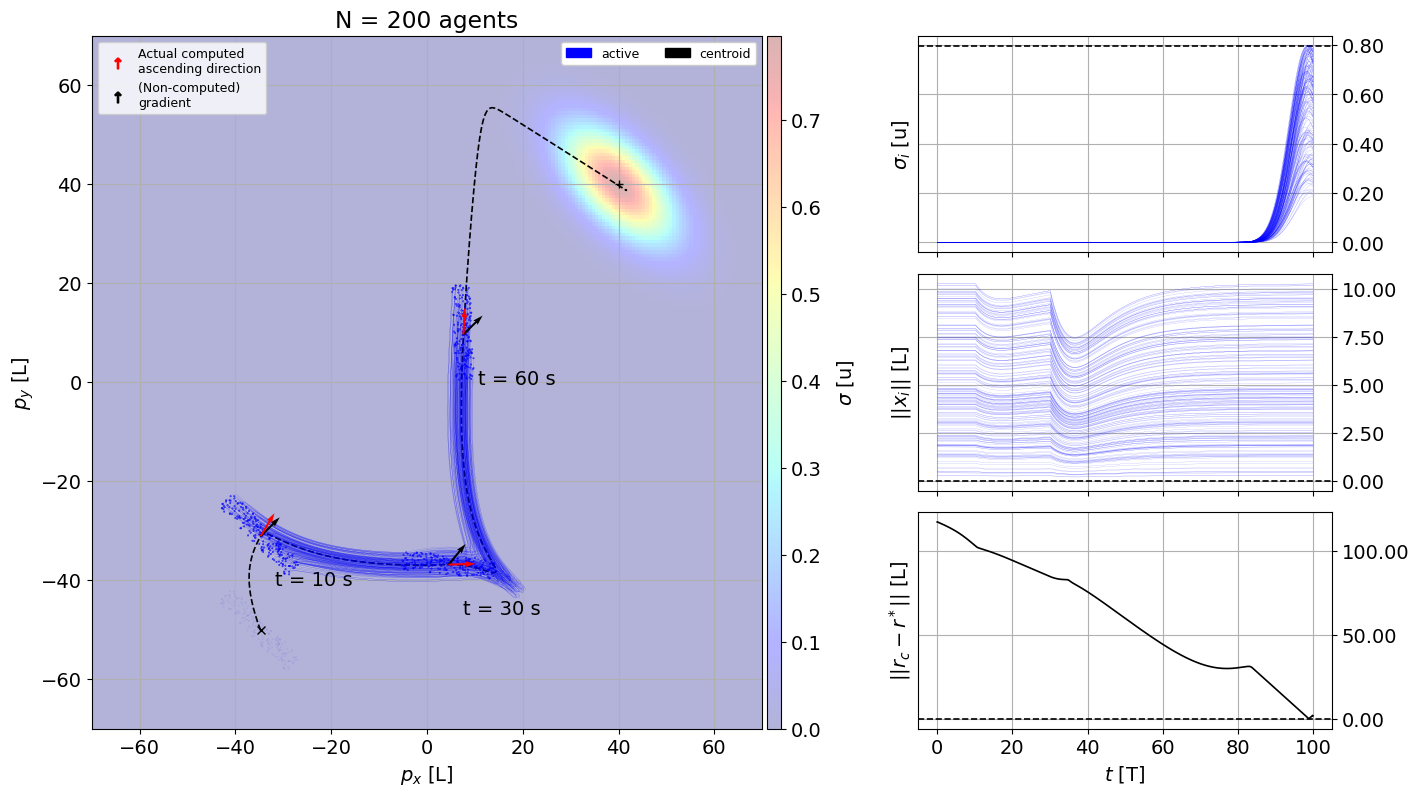
\includegraphics[trim={0cm 0.0cm 0cm 0.0cm}, clip, width=1\columnwidth]{./fig/ss_sim3.png}
\caption{En esta figura tenemos la simulación (III) de un enjambre de robots ejecutando nuestro algoritmo de \textit{source-seeking}. En el gráfico de la izquierda tenemos una representación del escenario virtual que permite visualizar cómo se aproxima el enjambre a la fuente a la vez que rota su formación; mientras que en los gráficos de la derecha se visualiza la distancia del centroide a la fuente y, para todo agente $i$, la medición $\sigma_i$ y su distancia al centroide $x_i$.}
\label{fig: ss_sim3}
\end{figure}

\subsubsection*{Sim. IV: Enjambre con formación tipo Batman controlado por un campo escalar que rota}

La cuarta misión (\autoref{fig: ss_sim4}) que proponemos en esta sección es muy peculiar. Tenemos a un enjambre de 150 agentes, distribuido uniformemente en los bordes de una formación que se asemeja al logo de Batman (igual que en la \autoref{fig: batman}), que debe encontrar la fuente de una señal gaussiana con simetría elíptica variante en el tiempo. 

En esta simulación, se intenta enfatizar más todavía en el potencial de maniobrabilidad del que dispone nuestro algoritmo. En este caso, el campo es generado y modulado por un agente externo, por lo que se puede interpretar como un \textbf{campo de control}; es decir, una herramienta de control sobre el enjambre. A partir de t = 20, se puede observar cómo la dirección de movimiento del enjambre rota según lo hace el propio campo.

Este es un resultado numérico con un enorme potencial, pues puede llegar a ser el origen de una nueva metodología para guiar a enjambres de robots de forma controlada, resiliente y robusta. Por ejemplo, imaginemos que tenemos una red de equipos capaces de generar un campo de control sobre sus vecinos; además, supongamos que el equipo 1 puede comunicarse con el 2 y el 2 con el 3. En este escenario, dada una situación en la que el equipo 1 se encuentra en rumbo de colisión con el 3, el equipo 2 podría generar un campo de control para guiar al equipo 1 hasta una zona segura.

\begin{figure}[!h]
\centering
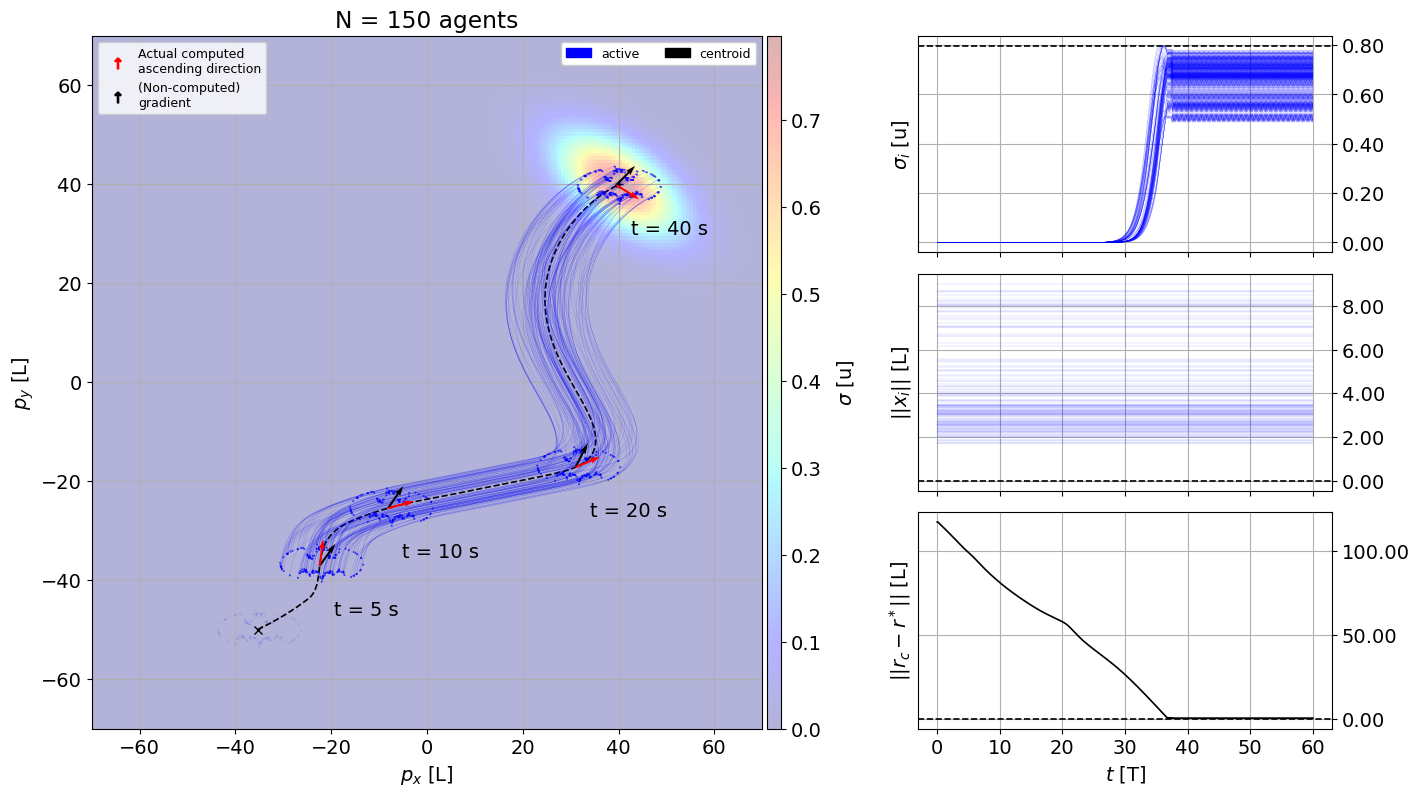
\includegraphics[trim={0cm 0.0cm 0cm 0.0cm}, clip, width=1\columnwidth]{./fig/ss_sim4.png}
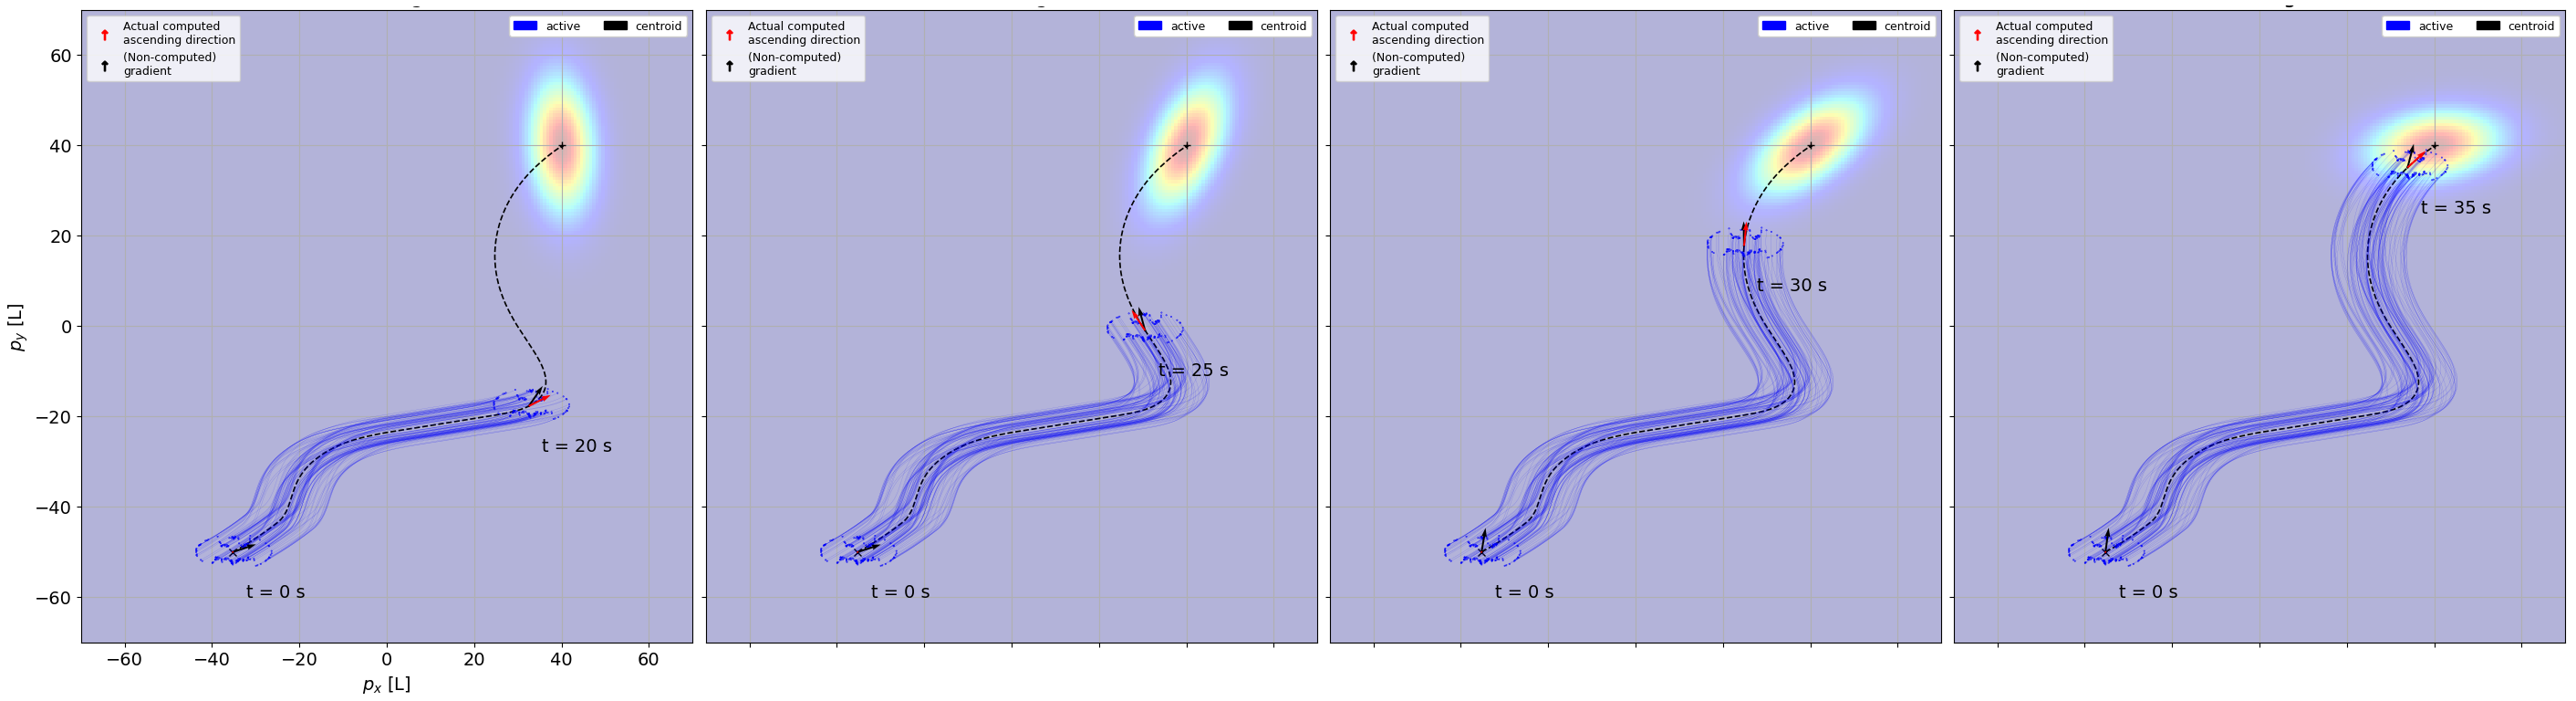
\includegraphics[trim={0cm 0.0cm 0cm 0.0cm}, clip, width=1\columnwidth]{./fig/ss_sim4_rot.png}
\caption{En esta figura tenemos la simulación (IV) de un enjambre de robots ejecutando nuestro algoritmo de \textit{source-seeking}. En el gráfico de la izquierda tenemos una representación del escenario virtual que permite visualizar cómo se aproxima el enjambre a la fuente de un campo que está rotando; mientras que en los gráficos de la derecha se visualiza la distancia del centroide a la fuente y, para todo agente $i$, la medición $\sigma_i$ y su distancia al centroide $x_i$. Las cuatro capturas de la simulación que aparecen en la parte inferior de la figura intentan visualizar cómo rota entre t = 20 y t = 35.}
\label{fig: ss_sim4}
\end{figure}

\newpage

\subsubsection*{Sim. V: Un enjambre de uniciclos en busca de la fuente de un campo cuadrático}

En esta quinta misión (\autoref{fig: ss_sim5}), contamos con un enjambre, compuesto esta vez por 20 \textbf{uniciclos}, que debe de encontrar la fuente de un campo escalar cuadrático. Este caso es mucho más particular que los anteriores, pues ahora la dinámica de los robots no nos permite tomar directamente $\dot x = \hat L_\sigma$. No obstante, en \cite{tfg_antonio} se demuestra que es posible implementar un controlador similar al utilizado en \cite{gvf_classic} para alinear a los robots con $L_\sigma$.

El objetivo de esta simulación es demostrar numéricamente que nuestro algoritmo de \textit{source-seeking}, también funciona para dinámicas más realistas. Este caso es tan interesante porque dinámica de muchos sistemas reales pueden aproximarse a la de un uniciclo, como los aviones de ala fija (\textit{fixed-wing}) o los vehículos con volante (\autoref{subsubsec: rover_dyn}).

\newpage

\begin{figure}[!h]
\centering
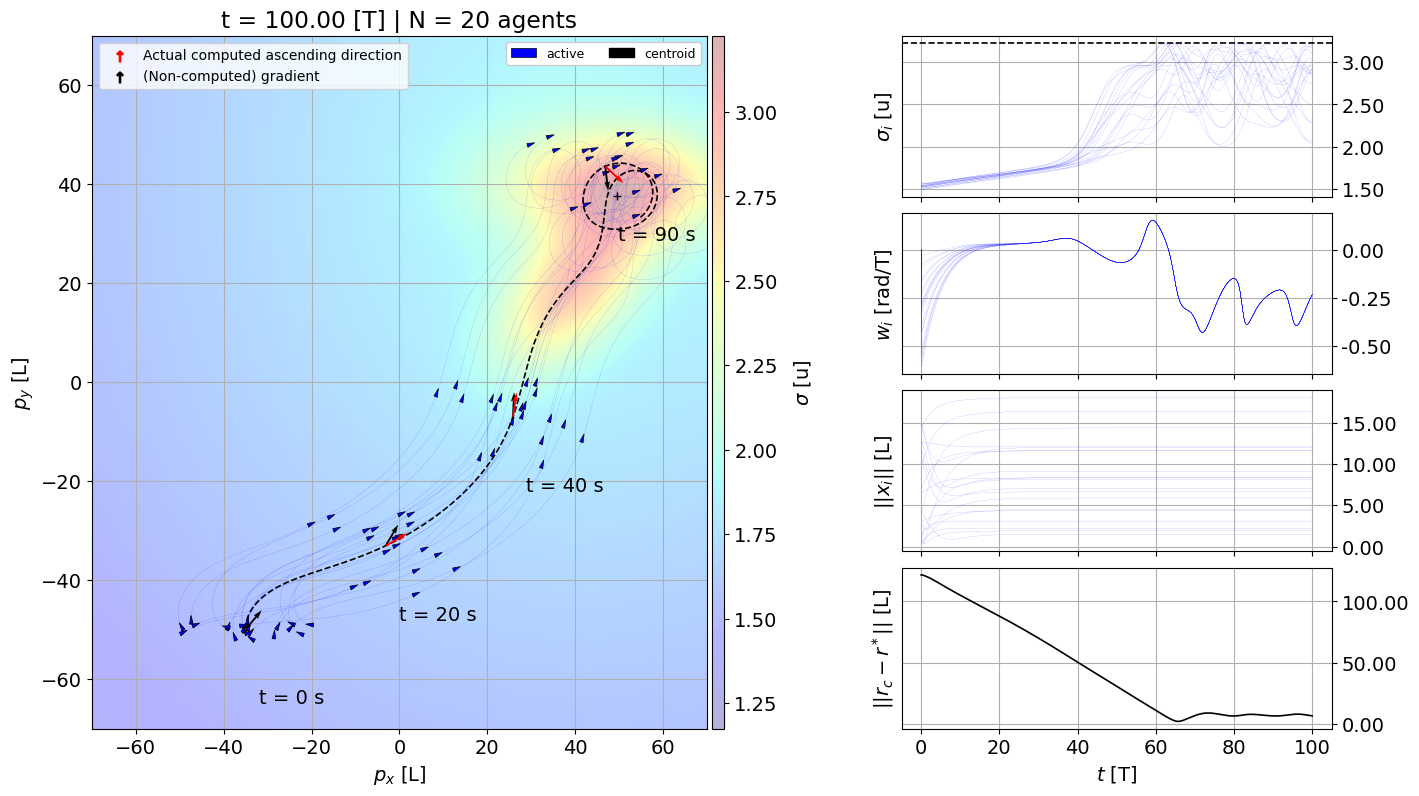
\includegraphics[trim={0cm 0.0cm 0cm 0.0cm}, clip, width=1\columnwidth]{./fig/ss_sim5.png}
\caption{En esta figura tenemos la simulación (V) de un enjambre de unicilos ejecutando de forma coordianada nuestro algoritmo de \textit{source-seeking}. En el gráfico de la izquierda tenemos una representación del escenario virtual que permite visualizar cómo se aproximan los enjambre a la fuente; mientras que en los gráficos de la derecha se visualiza la distancia del centroide a la fuente y, para todo agente $i$, la medición $\sigma_i$, su velocidad angular $\omega_i$ y su distancia al centroide $x_i$.}
\label{fig: ss_sim5}
\end{figure}

\subsubsection*{Sim. VI: Dos equipos se fusionan para evitar colisionar mientras se aproximan a la fuente}

En esta sexta y última misión (\autoref{fig: ss_sim6}), tenemos a dos enjambres de uniciclos, cada uno compuesto por 15 agentes distribuidos de forma aleatoria, que deben encontrar la fuente de un mismo campo cuadrático. Dado que ambos equipos se van a dirigir al mismo punto, llegará un momento en el que tengan que fusionarse para evitar colisionar entre ellos.

El objetivo de esta simulación es demostrar que nuestro algoritmo es capaz de gestionar la fusión de varios equipos en un solo enjambre (t = 60). A efectos prácticas, esta última misión es equivalente a la primera (\autoref{fig: ss_sim1}), ya que la fusión y separación de varios clusters es equivalente a introducir o desconectar agentes de la red. La mayor complicación reside en coordinar a las unidades de cómputo para que calculen una dirección de ascenso común; no obstante, en el Colorario \ref{cor: clus} ya demostramos que es posible y ahora ha quedado verificado numéricamente.

En el contexto de utilizar la fusión de enjambres para evitar colisiones, resulta pertinente pensar en cómo identificar que los enjambres se encuentran en rumbo de colisión. En este caso, sería interesante retomar las herramientas introducidas en la metodología anterior, y diseñar una CBF válida capaz de identificar de forma robusta cuándo dos direcciones de ascenso $L_\sigma$ están en conflicto.

\newpage

\begin{figure}[!h]
\centering
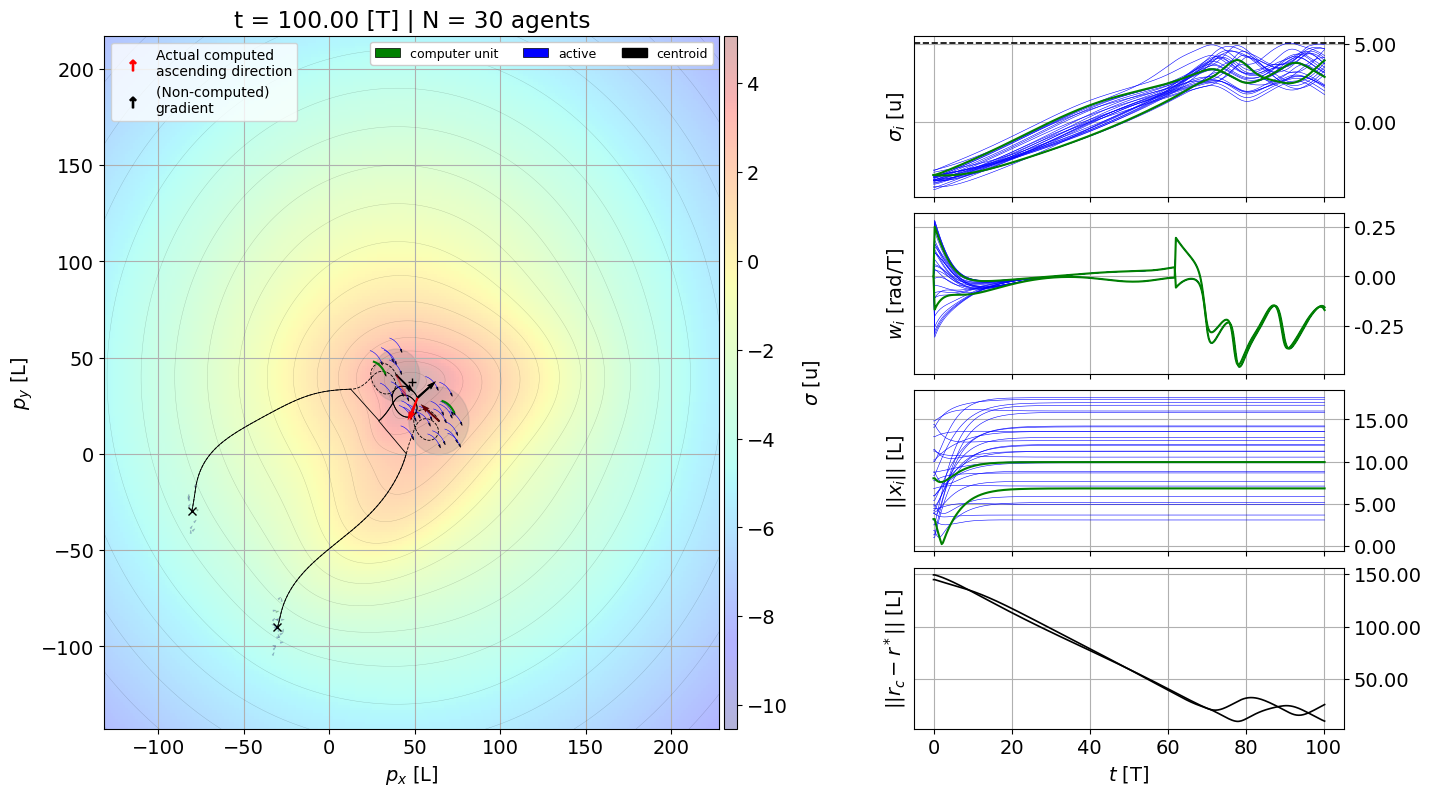
\includegraphics[trim={0cm 0.0cm 0cm 0.0cm}, clip, width=1\columnwidth]{./fig/ss_sim6.png}
\caption{En esta figura tenemos la simulación (V) de dos uniciclos de robots ejecutando de forma coordianada nuestro algoritmo de \textit{source-seeking}. En el gráfico de la izquierda tenemos una representación del escenario virtual que permite visualizar cómo se aproximan los enjambre a la fuente; mientras que en los gráficos de la derecha se visualiza la distancia del centroide a la fuente y, para todo agente $i$, la medición $\sigma_i$, la velocidad angular $\omega_i$ y su distancia al centroide $x_i$.}
\label{fig: ss_sim6}
\end{figure}


%%%%%%%%%%%%%%
% Conclusión %
%%%%%%%%%%%%%%

\subsection{Conclusiones}

En esta metodología, nos hemos centrado en analizar una nueva forma de resolver el problema de \textit{source-seeking} con enjambres de robots, propuesta originalmente en \cite{tfg_antonio}. Una solución que, en contraposición con los métodos ya existentes, es capaz de trabajar con geometrías genéricas de la formación, gracias al cómputo una dirección de ascenso. En este trabajo, hemos analizado en profundidad la observabilidad y sensibilidad de dicha dirección de ascenso, proponiendo una serie de resultados teóricos que han permitido identificar varias herramientas para maniobrar al enjambre mientras éste se sigue aproximando a la fuente. Además, en vista a implementar estas técnicas en una flota real de robots, también se ha propuesto un algoritmo capaz de estimar el centroide de forma distribuida, lo cual respeta la filosofía de enjambre.

De cara a un trabajo futuro, se puede puede pensar en diseñar un experimento que nos permita verificar todos estos resultados sobre un enjambre real. Adicionalmente, aprovechando las propiedades de nuestro algoritmo, se podrían explorar nuevas soluciones para algunos de los grandes problemas actuales dentro de la robótica de enjambre, como la integración local de múltiples equipos basada en las cuatro C's (coordinación, cooperación, colaboración y competición) o la evasión de colisiones.

